\documentclass[twoside,11pt]{article}

% Any additional packages needed should be included after jmlr2e.
% Note that jmlr2e.sty includes epsfig, amssymb, natbib and graphicx,
% and defines many common macros, such as 'proof' and 'example'.

% Available options for package jmlr2e are:
%   - abbrvbib : use abbrvnat for the bibliography style
%   - nohyperref : do not load the hyperref package
%   - preprint : remove JMLR specific information from the template,
%         useful for example for posting to preprint servers.

\usepackage[preprint]{mint2e}  % Using preprint option for flexibility

% Additional packages for your research
\usepackage{amsmath}
\usepackage{amsfonts}
\usepackage{booktabs}
\usepackage{url}
\usepackage{hyperref}
\usepackage{array}
\usepackage{longtable}
\usepackage{subfig}
\usepackage{graphicx}
\usepackage{subcaption}
\usepackage{xcolor}

% Definitions of handy macros
\newcommand{\dataset}{{\cal D}}
\newcommand{\fracpartial}[2]{\frac{\partial #1}{\partial  #2}}

% Heading arguments are {volume}{year}{pages}{date submitted}{date published}{paper id}{author-full-names}
\usepackage{lastpage}
\jmlrheading{}{2025}{1-\pageref{LastPage}}{Date submitted}{Date published}{25-0000}{Authors}

% Short headings should be running head and authors last names
\ShortHeadings{MINT: Multi-participant Interactive Trading}{Authors}
\firstpageno{1}

\begin{document}

\title{MINT: Multi-participant Interactive Trading for Experimental Economics}

\author{\name Authors \email authors@university.edu \\
       \addr Department of Economics\\
       University Name\\
       City, State, Country}

\editor{Editor Name}

\maketitle

% Include abstract
\begin{abstract}
We present MINT (Multi-participant Interactive Trading), a platform for experimental economics research enabling multi-participant trading sessions with role-based assignments. The system features event-driven architecture, session pool management, and integration of human participants with algorithmic traders. The platform implements lazy market creation that reduces resource consumption, WebSocket communication, and data collection across over 40 parameters. The system supports authentication methods including Prolific integration for research. MINT enables investigation of strategic interactions, information transmission, and market microstructure effects in experimental environments. The software is provided as open-source to encourage research community adoption.
\end{abstract}

\begin{keywords}
  experimental economics, trading platform, market microstructure
\end{keywords}

\newpage

\tableofcontents

\newpage

% Include introduction
\section{Introduction}

\subsection{Background and Motivation}

\subsection{Experimental Trading Platforms}

Experimental trading platforms have changed significantly, moving from simple laboratory tools to flexible web-based systems that researchers can use for many different studies \citep{Andraszewicz2023Zurich, Chen2016oTree, Cliff2018Open}. Researchers needed better tools that could handle complex market behavior while still providing the accuracy needed for studying how people behave in financial markets.

\subsubsection{Evolution from Traditional to Modern Platforms}

Most early researchers used zTree \citep{fischbacher2007z} for their trading experiments. While zTree was important for economics research, it had serious limitations - it couldn't handle complex markets very well, and researchers needed programming skills to create trading environments \citep{Fischbacher1999z}. To work around these problems, researchers created add-ons for online experiments \citep{Ertac2020z} and tools for studying preferences \citep{Fidanoski2022Z}.

Web-based platforms changed what researchers could do. oTree \citep{Chen2016oTree} used Python programming, which made it much easier to build new experiments and run them both in labs and online. Because oTree was more flexible, researchers built many add-ons, including better communication systems using websockets \citep{Crede2019Otree, Washinyira2023Integrating} and market simulation tools \citep{Grant2020oTree}. oTree worked particularly well for double auctions and trading experiments \citep{Aldrich2019oTree}.

Researchers also built specialized trading platforms for specific needs. The Bristol Stock Exchange (BSE) \citep{Cliff2018Open} focused on limit order books for trading research. Exchange Portal (ExPo) \citep{Stotter2014Behavioural} let researchers run experiments with both human participants and computer algorithms. GIMS \citep{Palan2015GIMSSoftware} provided tools for market experiments, while ABIDES \citep{Shi2023Neural} added computer modeling for simulating many different trading agents.

\subsubsection{Technical Capabilities and Methodological Advances}

Modern trading platforms can do things that older systems couldn't. Better communication technology, especially websockets, allows markets to update instantly and removes the delays that made earlier experiments unrealistic \citep{Crede2019Otree, Washinyira2023Integrating}. This means researchers can run more realistic trading simulations with proper market timing.

Many platforms now use agent-based modeling, where computer programs simulate different types of traders with various strategies \citep{Cliff2019Exhaustive, Snashall2019Adaptive}. The Bristol Stock Exchange and similar platforms have shown they're good at testing trading strategies and measuring performance in realistic market conditions \citep{Cliff2020Methods}. Recent improvements include studying how trader opinions spread \citep{Lomas2021Exploring, Bokhari2022Studying}, economic modeling, and understanding how order imbalances affect markets \citep{Zhang2020Market}.

Modern platforms are built to be modular, which means researchers can easily change how markets work, how traders behave, and how the system operates without having to rewrite the entire platform \citep{Aldrich2019oTree, Chen2016oTree}. Most platforms now use Python programming language, which makes it easier to build prototypes quickly and connect with other computer systems \citep{Mascioli2024Financial}.

\subsubsection{Application Domains and Research Impact}

These trading platforms help researchers study many different topics in finance, including how people behave in markets, how market structure affects trading, and how to evaluate trading strategies. Researchers have used these platforms to study how well trading algorithms perform \citep{Cliff2020Methods}, how to detect market manipulation \citep{Shi2023Neural}, how arbitrage works \citep{Sylvester2022Modeling}, and how people trade emissions permits \citep{Huang2015Experimental}. Adding machine learning and reinforcement learning to these platforms has created new opportunities for studying automated trading strategies \citep{Mascioli2024Financial}.

These applications have been very useful. For example, BSE works well for both research and teaching \citep{Cliff2018Open}. Because researchers can control the experimental environment completely, they can properly test trading strategies and market mechanisms under controlled conditions.

\subsubsection{Research Gaps and Limitations}

However, current trading platforms still have two important problems. First, most platforms make it very difficult for researchers to add new types of traders without rewriting large parts of the system, which limits how flexible experiments can be and makes it hard to test new behavioral models. Second, many platforms can't record detailed data about what happens during experiments, so researchers miss important information about how market conditions change and how participants make decisions while trading.

\subsection{Platform Design Objectives}


% Include methodology (related work + platform architecture)
\section{Platform Design}
\label{sec:platform}

This section explains how we built our trading platform that can handle multiple participants at once. The platform has over 40 settings that researchers can adjust to control how the market works, how traders behave, and what experimental conditions to test. We provide all the parameter details with their mathematical symbols and default values in Appendix~\ref{app:parameters}.

\subsection{Market Structure}
\label{sec:market}

Our experimental market includes both human participants $\mathcal{N} = \{1, 2, \ldots, n\}$ and computer-controlled agents $\mathcal{A} = \{n+1, n+2, \ldots, m\}$. The human participants can be either informed traders $\mathcal{N}_I \subset \mathcal{N}$ or speculators. The computer agents include informed traders $\mathcal{A}_I \subset \mathcal{A}$ and noise traders $\mathcal{A}_N \subset \mathcal{A}$. Trading happens continuously over time from start $[0, \tau]$ where $\tau$ is how long the market stays open.

The platform keeps track of all buy orders $\mathbf{B}_t$ and sell orders $\mathbf{A}_t$ separately. Each order $o_i = (p_i, q_i, t_i)$ contains the price, quantity, and time when trader $i$ submitted it. When multiple orders have the same price, we combine their quantities. Orders execute immediately when the highest buy price meets or exceeds the lowest sell price:
\begin{equation}
\max(\mathbf{B}_t) \geq \min(\mathbf{A}_t)
\end{equation}

The platform keeps track of when each trader $i \in \mathcal{N} \cup \mathcal{A}$ places orders to ensure fair trading and accurate data recording.

\subsection{Parallel Market Creation}
\label{sec:sessions}

The platform can run multiple markets at the same time to collect data from different groups of participants. We call these parallel markets $\mathcal{M} = \{M_1, M_2, \ldots, M_j\}$, where each market $M_j$ works independently with its own group of participants $\mathcal{N}_j \subset \mathcal{N}$.

Participants join waiting pools $\mathcal{S}_s$ that have a fixed capacity $\nu_s = |\mathbf{g}|$, where $\mathbf{g} = [g_1, g_2, \ldots, g_{\nu_s}]$ is a list of trading goals we set up ahead of time. These goals tell participants what they should try to do: positive numbers mean they should buy that many shares, negative numbers mean they should sell that many shares, and zero means they should just try to make profit without specific targets. For example, if we set $\mathbf{g} = [100, -50, 0]$, we get one buyer (who should buy 100 shares), one seller (who should sell 50 shares), and one speculator.

We assign roles based on position in the pool: participant $k$ in pool $\mathcal{S}_s$ gets goal $g_k$ and role $r_k$ where:
\begin{equation}
r_k = \begin{cases}
\text{INFORMED} & \text{if } g_k \neq 0 \\
\text{SPECULATOR} & \text{if } g_k = 0
\end{cases}
\end{equation}

A new market starts when the waiting pool fills up completely ($|\mathcal{S}_s| = \nu_s$), which creates market $M_j$ with all the trading features ready to go. This wait-until-full approach lets us collect data from multiple independent markets running at the same time.

\subsection{Order Book Initialization}

Before participants join the market, the platform automatically places some initial orders to provide liquidity. This setup fills both the buy side $\mathbf{B}_0$ and sell side $\mathbf{A}_0$ of the order book with a predetermined number of orders.

For the initial buy orders, we randomly generate prices $p^{buy}_k$ from the range $[p_0 - \ell \cdot \sigma, p_0 - \sigma]$ for $k = 1, \ldots, \ell \times \omega$. For the initial sell orders, we generate prices $p^{sell}_k$ from the range $[p_0 + \sigma, p_0 + \ell \cdot \sigma]$. We then sort these prices so that:
\begin{align}
p^{buy}_1 \geq p^{buy}_2 \geq \cdots \geq p^{buy}_{\ell \times \omega} \\
p^{sell}_1 \leq p^{sell}_2 \leq \cdots \leq p^{sell}_{\ell \times \omega}
\end{align}

Each initial order has a quantity of $q = 1$, which creates balanced market depth on both sides around the starting price $p_0$ before human traders $\mathcal{N}$ start trading.

\subsection{Trader Endowments}

The market trades one asset (shares) for cash. We give traders different starting amounts of cash and shares depending on their type and the goals we assigned them in the session pools. Table~\ref{tab:endowments} summarizes the initial resource allocation across trader types.

\begin{table}[ht]
\centering
\caption{Initial Endowments by Trader Type}
\label{tab:endowments}
\begin{tabular}{llll}
\toprule
Trader Type & Cash & Shares & Rationale \\
\midrule
Human Participants & $C_0$ & $S_0$ & Equal starting conditions regardless of goal $g_i$ \\
Noise Traders & $\infty$ & $\infty$ & Continuous liquidity provision \\
Informed (Buyers) & $2g_i \cdot p_0$ & $0$ & Sufficient cash to complete purchases \\
Informed (Sellers) & $0$ & $g_i$ & Exact shares needed to fulfill goal \\
\bottomrule
\end{tabular}
\end{table}

All human participants start with identical resources $(C_0, S_0)$ regardless of their assigned goals $g_i$, with initial portfolio value $W_0 = C_0 + S_0 \cdot p_0$. This ensures that success depends on trading strategy rather than differential initial endowments. Computer agents receive resources tailored to their market roles: noise traders operate with unlimited resources to maintain continuous market activity, while informed traders receive goal-matched allocations where $g_i$ represents their target trading amount.

\subsection{Price Formation}

Market prices come from how participants trade with each other - there's no external price setting. The mid-price at time $t$ is the average of the best buy price and best sell price:
\begin{equation}
p_{mid,t} = \frac{\min(\mathbf{A}_t) + \max(\mathbf{B}_t)}{2}
\end{equation}

The bid-ask spread $s_t$ tells us how liquid the market is (smaller spreads mean more liquid):
\begin{equation}
s_t = \min(\mathbf{A}_t) - \max(\mathbf{B}_t)
\end{equation}

When the market closes, we need to deal with any orders that haven't executed yet so we can calculate final portfolio values and pay participants. The closure system makes sure everyone gets a definite payoff even if they have unfilled orders. For any remaining order with quantity $q$, we calculate closure prices as:
\begin{align}
p_{closure}^{buy} &= p_{mid,\tau} + q \cdot \Delta \cdot \kappa \\
p_{closure}^{sell} &= p_{mid,\tau} - q \cdot \Delta \cdot \kappa
\end{align}
where $\Delta$ is the default spread width and $\kappa$ is a penalty factor that makes larger orders more expensive. This pricing gives worse prices than normal market trading to discourage people from gaming the system by placing strategic orders right before the market closes.

\section{Trader Types}

\subsection{Human Traders}

Human traders make discrete choices about their orders. When trader $i$ wants to place an order at time $t$, they choose from available options $\mathcal{O}_i(t) = \{(p, q, \theta) : p \in \mathbb{R}^+, q \in \mathbb{N}, \theta \in \{-1, 1\}\}$ where $p$ is price, $q$ is quantity, and $\theta$ is whether it's a buy (+1) or sell (-1) order. The platform shows them pre-calculated price levels $P_t^{buy}, P_t^{sell}$ based on current best prices to help them make decisions quickly.

For informed traders $i \in \mathcal{N}_I$, we track how close they are to completing their goals by adding up their executed trades:
\begin{equation}
\pi_i(t) = \sum_{s=0}^{t} q_{i,s} \cdot \text{sign}(g_i)
\end{equation}
where $q_{i,s}$ is how much they traded at time $s$, and they complete their goal when $\pi_i(t) \geq |g_i|$.

The platform can optionally coordinate timing between human participants and computer traders. When this feature is turned on, human trading gets paused while computer traders are active, which prevents interactions that might mess up the experimental results. Researchers can choose whether to use this feature depending on their experimental design.

\subsection{Noise Traders}

Noise traders create background market activity using unlimited money and shares to keep the market liquid. Each time they act, they first might cancel an existing order (with probability $\epsilon$), then they place a new order.

Noise traders usually decide between buying and selling with probability $\zeta$ for buys. But they have a special rule: if there are no buy orders in the market, they only place buy orders; if there are no sell orders, they only place sell orders. This keeps both sides of the market active at all times.

When placing orders, noise traders choose between two types of trading:
\begin{align}
\mathbb{P}(\text{Passive}) &= \delta \\
\mathbb{P}(\text{Aggressive}) &= 1 - \delta
\end{align}

Passive orders add liquidity by placing orders at prices worse than the current best prices - these use prices $p = p_{best,t} \pm k \cdot \sigma$ where $k$ is a random distance from the best price, chosen from levels $\{1, 2, \ldots, \ell\}$. Aggressive orders consume liquidity by matching with existing orders at current market prices. Order sizes are chosen randomly up to a maximum of $q_{max}$ to make the trading look realistic.

\subsection{Informed Traders}

Informed traders use a conditional aggressive strategy that depends on how wide the spread is. They only trade when the current bid-ask spread $s_t$ is smaller than their edge parameter $\gamma$, where $\gamma$ is the maximum spread they're willing to pay. When $s_t \leq \gamma$, buying-oriented traders take the best sell price and selling-oriented traders take the best buy price. When $s_t > \gamma$, informed traders wait for the spread to narrow.

The platform can also let informed traders use passive strategies where they place limit orders at multiple price levels near the best prices, but the standard setup uses only the aggressive approach described above.

We set trading goals to match expected noise trader activity so the market stays balanced. The automatic goal calculation is:
\begin{equation}
g_i = \left\lfloor \frac{\beta}{1-\beta} \cdot \mathbb{E}[V_N] \right\rfloor
\end{equation}
where $\beta$ is how intense informed trading should be and $\mathbb{E}[V_N]$ is how much we expect noise traders to trade during the session. Informed traders stop trading when they complete their goals, which keeps the experiment controlled by preventing them from trading too much.

\subsection{Data Collection}

The platform records every trading action with precise timestamps, which lets researchers completely rebuild what happened in the market after the experiment. Instead of taking snapshots of the order book, we record each individual order placement, execution, and cancellation.

Each recorded event includes who the trader was, what the order details were, and exactly when it happened. From this sequence of events, researchers can rebuild everything about how the market evolved, including order book states, transaction histories, and participant portfolios at any moment during trading.

To rebuild the market, we replay the logged events in chronological order to reconstruct the market state $X_t = (\mathbf{B}_t, \mathbf{A}_t, p_{mid,t}, s_t, V_t)$ where $V_t$ is the total volume traded. We also track how each trader's cash and shares $(C_{i,t}, S_{i,t})$ changed over time for every trader $i \in \mathcal{N} \cup \mathcal{A}$. 

We calculate each trader's profit and loss using current market values:
\begin{equation}
\Pi_{i,t} = C_{i,t} + S_{i,t} \cdot p_{mid,t} - W_{i,0} \label{eq:pnl}
\end{equation}
where $W_{i,0}$ is what their portfolio was worth at the start.

\subsection{Platform Interface}
\label{sec:interface}

The platform gives participants a trading interface to make decisions in the electronic market. Understanding this interface is important because it determines how participants interact with the market systems we described above.

\subsubsection{Dashboard Layout}

The main trading interface has six information panels arranged in three columns, each serving different functions for trading, as shown in Figure~\ref{fig:dashboard}. The layout follows conventions from real financial trading platforms. Table~\ref{tab:dashboard} summarizes the panel organization and functionality.

\begin{table}[ht]
\centering
\caption{Trading Dashboard Panel Layout}
\label{tab:dashboard}
\begin{tabular}{p{0.18\textwidth}p{0.15\textwidth}p{0.55\textwidth}}
\toprule
Panel & Location & Key Information and Functionality \\
\midrule
Portfolio Header & Top & Role assignment ($\mathbf{g}$), P\&L ($\Pi_{i,t}$), share holdings ($S_{i,t}$) with change indicators, cash ($C_{i,t}$), active trader count, time remaining \\
\midrule
Trades History & Left-top & Completed transactions, volume-weighted average prices (VWAP$_{buy}$, VWAP$_{sell}$), executed trade details with timestamps \\
\midrule
Market Info & Left-bottom & Current transaction price, bid-ask spread, midpoint $p_{mid,t}$, noise trader status indicators \\
\midrule
Buy-Sell Chart & Center-top & Dual-sided bar chart showing bid-ask distribution, spread visualization with shading, real-time order book depth \\
\midrule
Passive Orders & Center-bottom & Unfilled limit orders with quantities and prices, management controls (+/- buttons) for order modification and cancellation \\
\midrule
Price History & Right-top & Transaction price evolution over time as line chart, trend visualization, market momentum indicators \\
\midrule
Trading Panel & Right-bottom & Order placement interface with buy/sell sections, price levels ($P_t^{buy}$, $P_t^{sell}$), execution buttons, role-based restrictions \\
\bottomrule
\end{tabular}
\end{table}

\begin{figure}[!htbp]
\centering
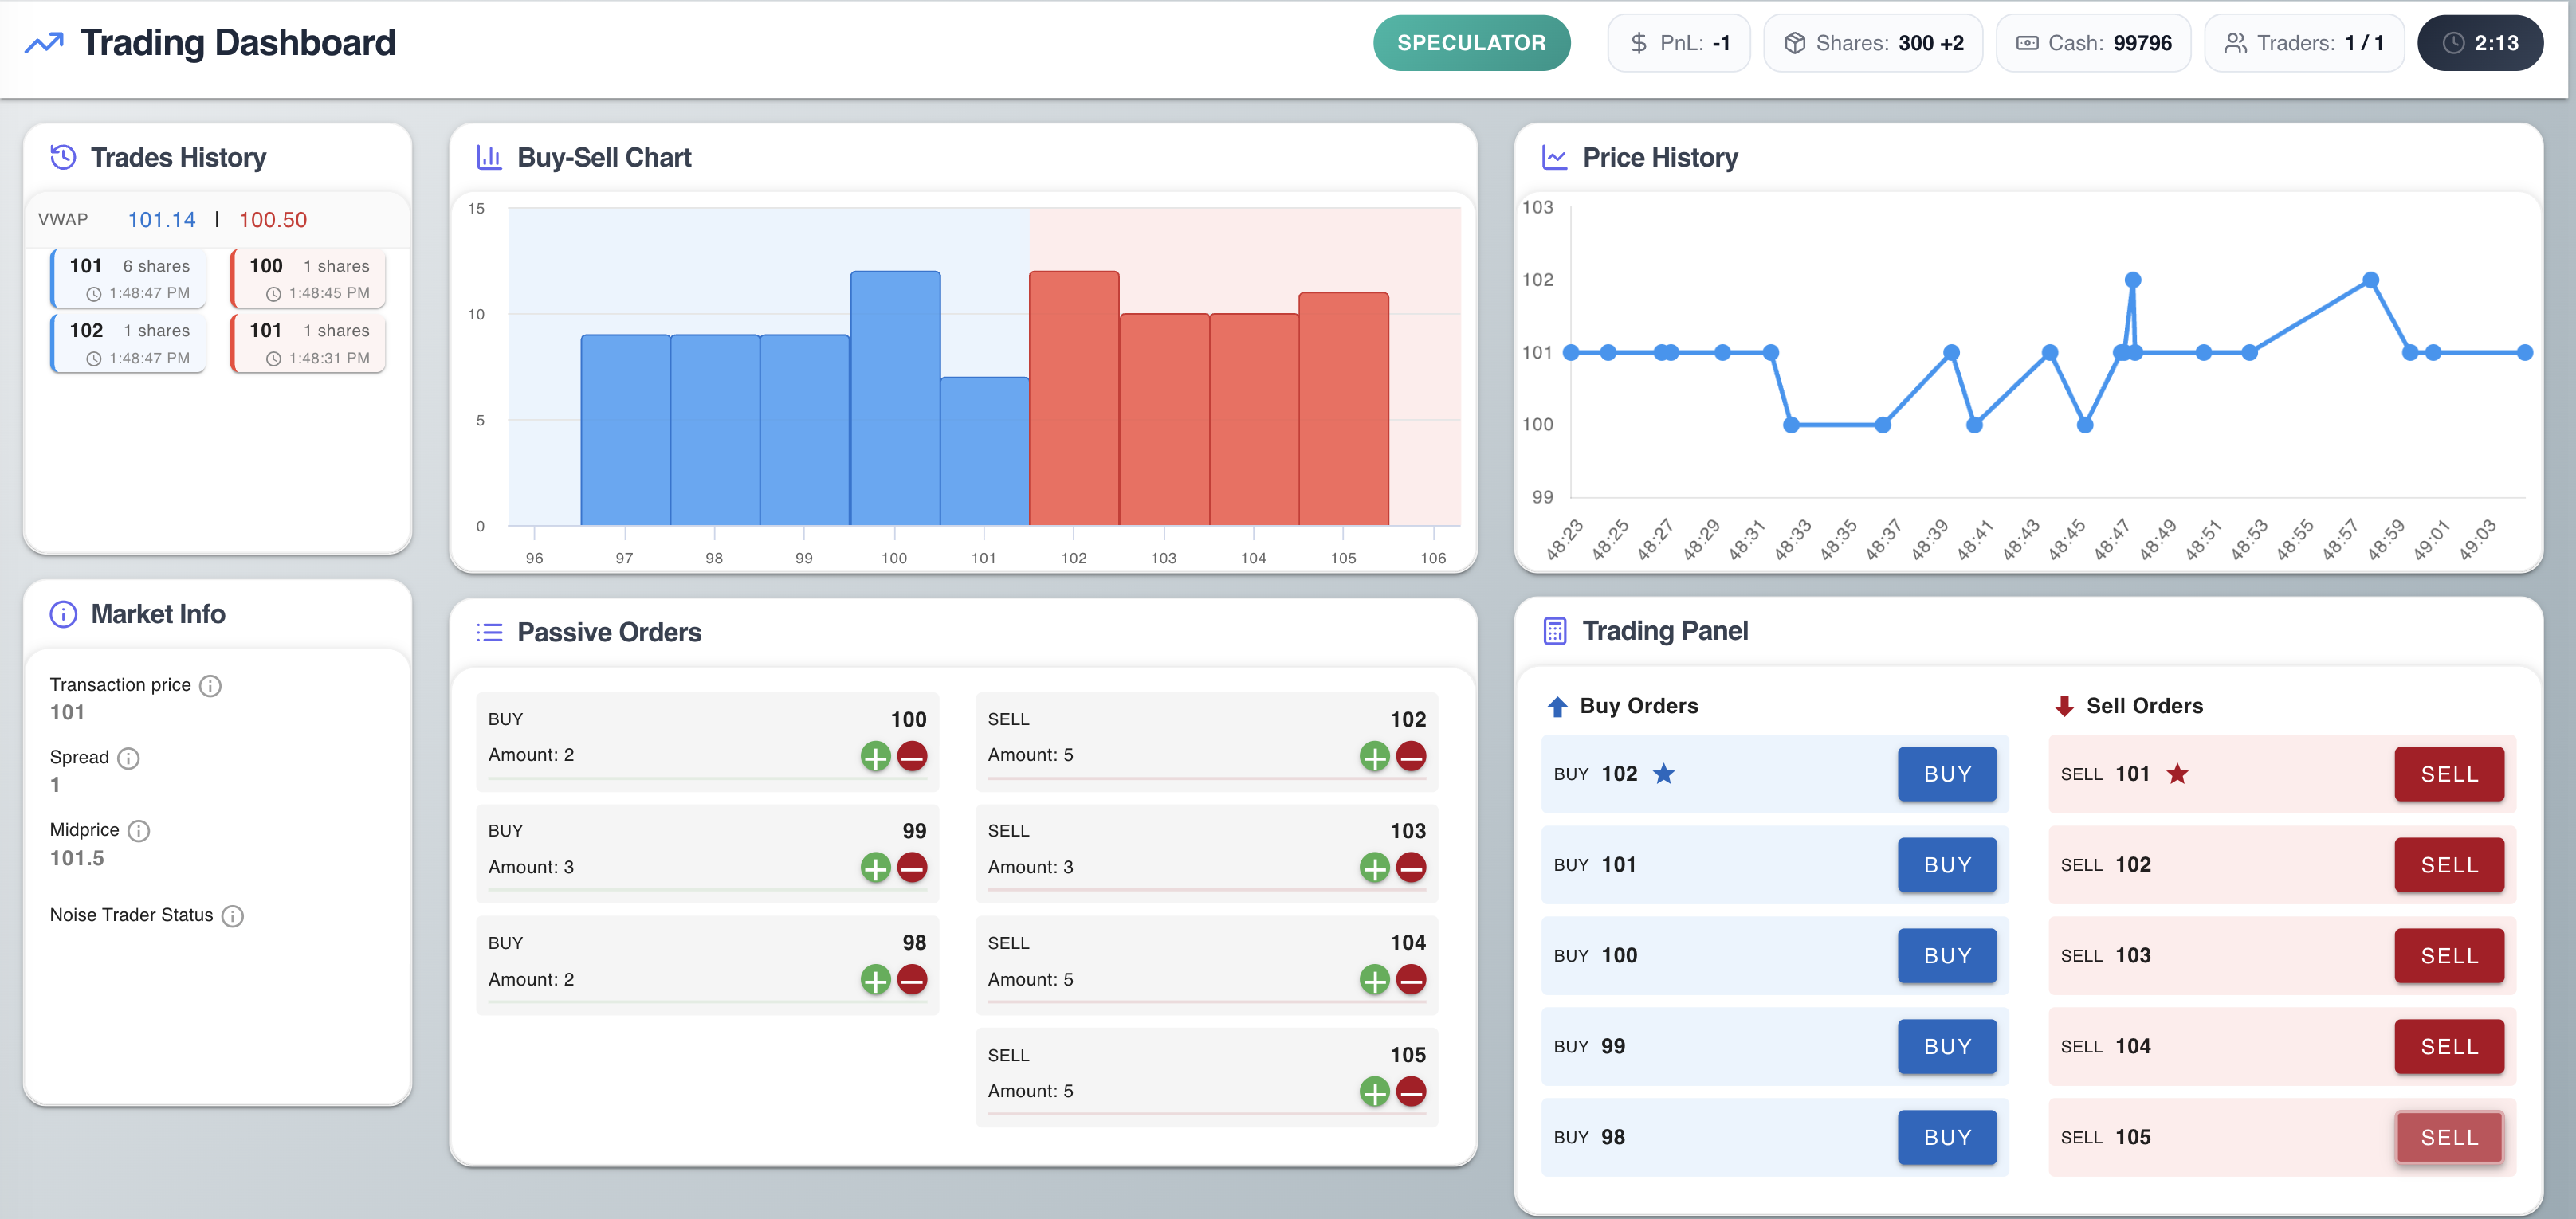
\includegraphics[width=0.95\textwidth]{figs/trading-dashboard.png}
\caption{Main Trading Interface. Six-panel layout showing trade history, market information, order book visualization, active orders, price history, and trading controls with portfolio status.}
\label{fig:dashboard}
\end{figure}

\subsubsection{Order Placement Interface}

The trading panel is in the right column and is where participants actually place their orders. It has two sections: one for buy orders and one for sell orders. Each section shows multiple price levels $P_t^{buy}$ and $P_t^{sell}$ with buttons that participants can click to execute trades.

The interface marks the best market prices with star icons. Depending on their assigned goals, some trading buttons are disabled: participants with $g_i > 0$ (buyers) cannot place sell orders, participants with $g_i < 0$ (sellers) cannot place buy orders, and all trading stops when they reach their goal $|\pi_i(t)| \geq |g_i|$ so the human trader can no longer place orders.

We calculate the price levels shown based on the current order book state $(\mathbf{B}_t, \mathbf{A}_t)$ and a step size parameter $\sigma$. The platform shows $\ell_{display}$ price levels above and below the current best prices. Order throttling parameters $\theta_{throttle}$ limit how fast participants can submit orders to prevent market manipulation.

When computer traders are active, pause notifications appear as banners on the screen, telling participants when human trading is temporarily disabled to prevent confusing interactions between human and computer trading strategies.

\subsubsection{Market Information Display}

The order book visualization occupies the center-left panel and presents bid-ask distribution as a dual-sided bar chart. Blue bars represent buy quantities at each price level, red bars show sell quantities. Background shading indicates the bid-ask spread region, with midpoint $p_{mid,t}$ marked.

The chart updates in real-time as orders are placed, executed, or cancelled, so participants can see how the market state changes. Through this visualization, participants can see how deep the market is and how liquid it is.

\subsubsection{Price History and Portfolio Tracking}

The price history chart (center-right panel) shows how transaction prices have changed over time using a line graph. Participants can see market trends and price momentum through this display.

The left column has two panels for managing portfolios. The active orders panel shows orders that haven't executed yet, and participants can add more orders at existing price levels or cancel orders using plus and minus buttons. The trade history panel shows completed transactions and calculates the volume-weighted average price (VWAP) for buy and sell trades:

\begin{align}
\text{VWAP}_{buy} &= \frac{\sum_{n} p_n \cdot q_n^{buy}}{\sum_{n} q_n^{buy}} \label{eq:vwap_buy}\\
\text{VWAP}_{sell} &= \frac{\sum_{n} p_n \cdot q_n^{sell}}{\sum_{n} q_n^{sell}} \label{eq:vwap_sell}
\end{align}

where $p_n$ and $q_n$ are the transaction prices and quantities for completed trades.

The interface provides tooltips to explain market information. Money amounts are shown in experimental currency units (Liras) with conversion rates to real compensation.

\subsubsection{Post-Market Summary Interface}

When the market closes, participants see a performance summary that shows statistics about the whole market and their individual trading performance, as shown in Figure~\ref{fig:summary}. The summary shows three types of information for analyzing the experiment and calculating participant compensation.

\begin{figure}[!htbp]
\centering
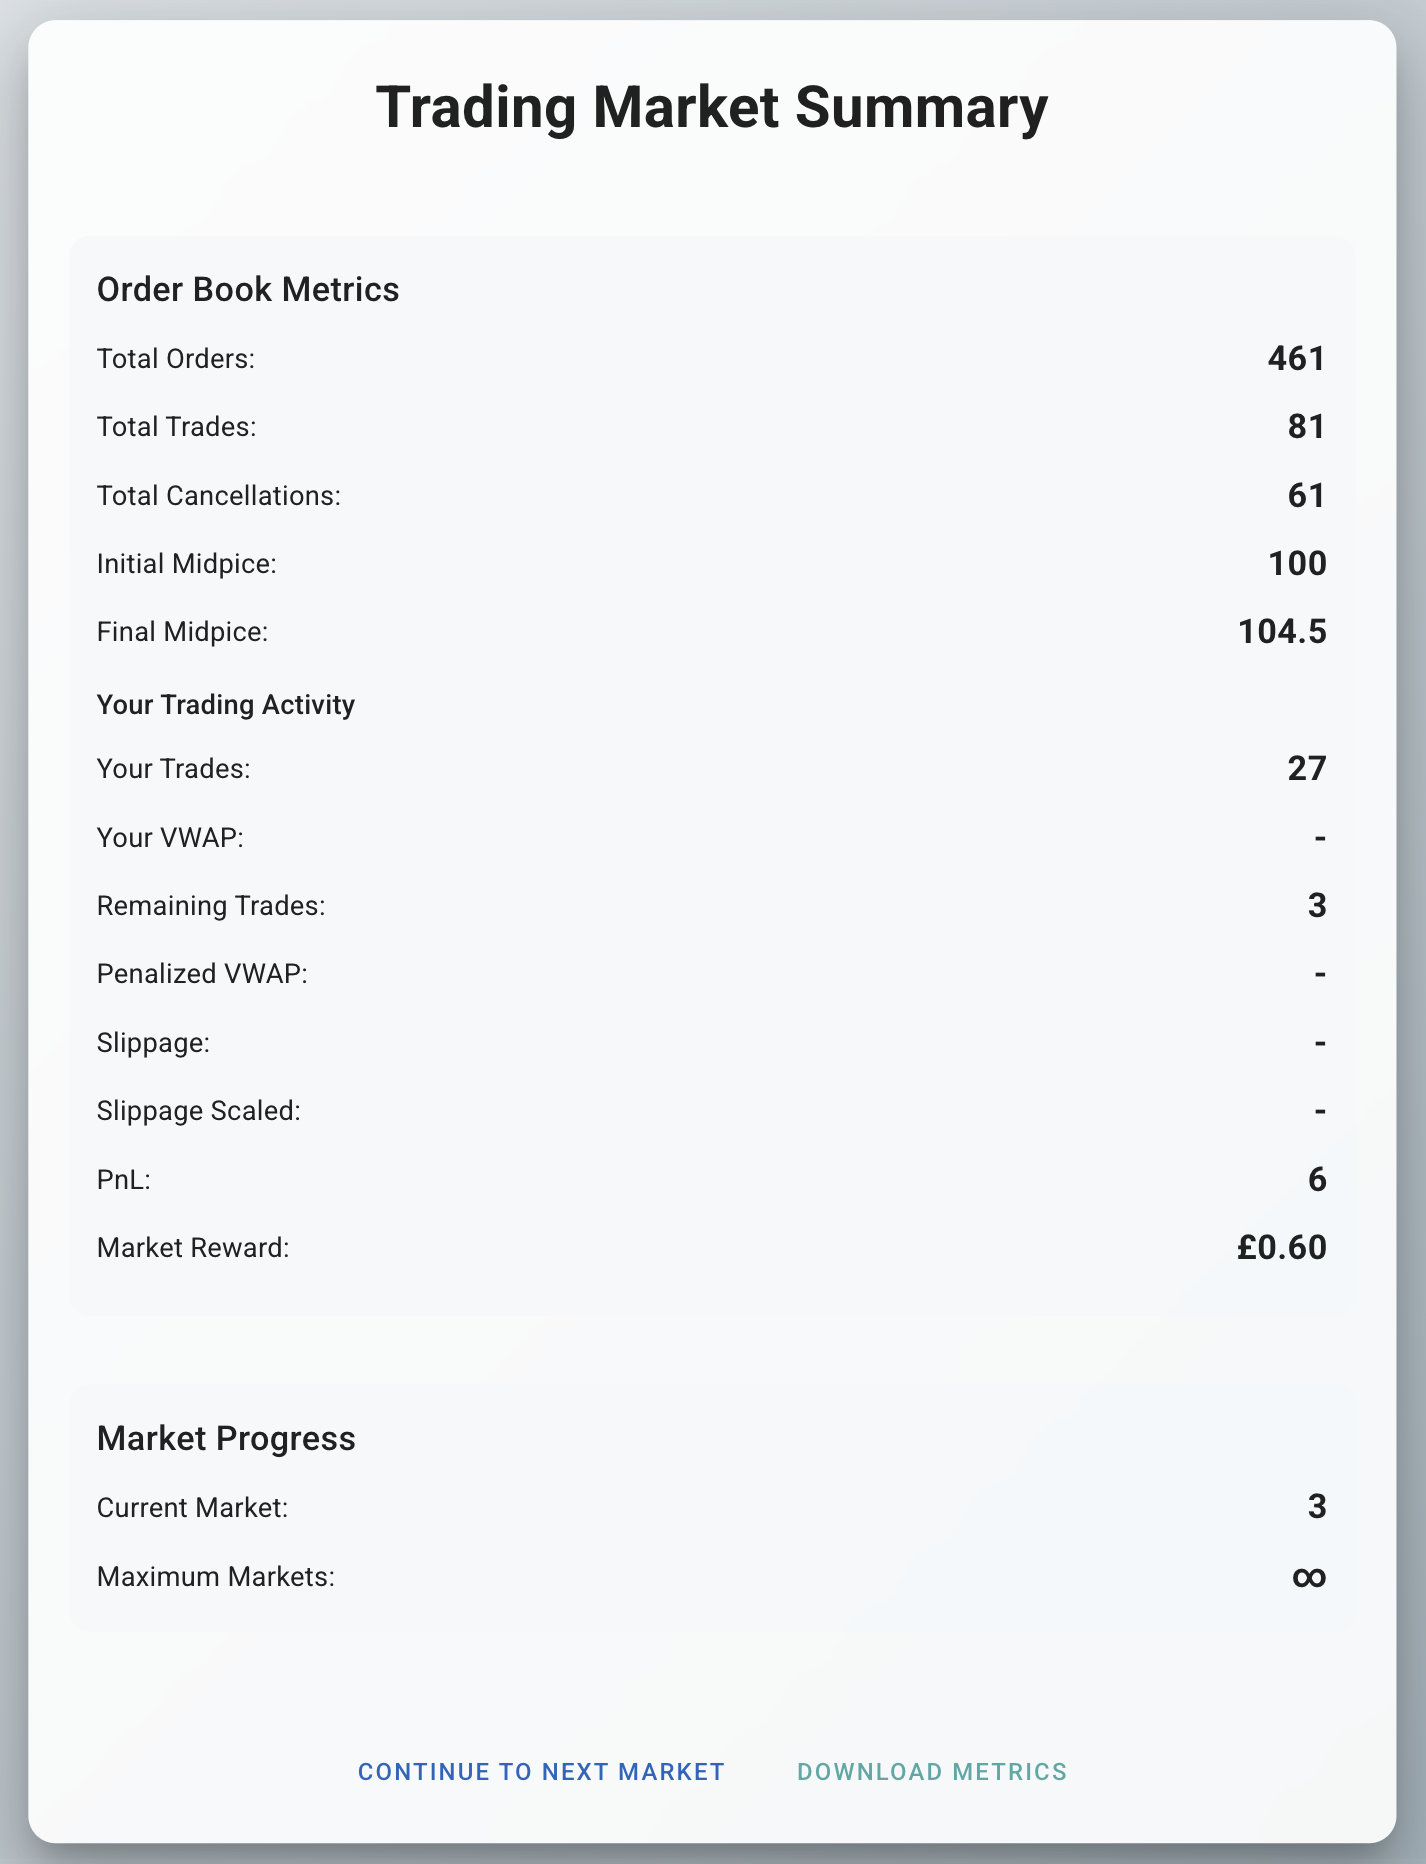
\includegraphics[width=0.7\textwidth]{figs/summary-page.png}
\caption{Post-Market Summary Interface. Trading metrics display including order book statistics, performance measures, and session progress with compensation calculations.}
\label{fig:summary}
\end{figure}

The Order Book Metrics section shows market-wide statistics that we reconstruct from the event log. Total orders, trades, and cancellations tell us how active the market was. The starting and ending midprices $p_{mid,0}$ and $p_{mid,\tau}$ show how price discovery worked during the trading session, which helps us assess market efficiency and price impact.

The Trading Activity section shows each trader's performance based on their assigned goals. The metrics include how many trades they completed, VWAP calculations using equations (\ref{eq:vwap_buy}) and (\ref{eq:vwap_sell}), and how many trades they still needed to complete their goals $g_i$. For participants who didn't complete their goals, the platform calculates penalized VWAP and slippage measures:

\begin{align}
\text{VWAP}_{penalized} &= \frac{\text{VWAP}_{actual} \cdot q_{executed} + p_{mid,\tau} \cdot \kappa \cdot q_{remaining}}{|g_i|} \label{eq:vwap_penalized}\\
\text{Slippage} &= \text{VWAP}_{penalized} - p_{mid,0} \label{eq:slippage}
\end{align}

where $q_{executed}$ is how many trades they completed, $q_{remaining} = |g_i| - q_{executed}$ is how many trades they still needed to complete their goal, and $\kappa$ is a penalty factor for not completing their target.

We calculate profit and loss using the mark-to-market method from equation (\ref{eq:pnl}), with portfolio values calculated when the market closes. We then convert trading performance into monetary compensation using performance-based scaling.

The Market Progress section keeps track of how participants advance through multiple experimental sessions. Market numbering and participation limits let researchers run repeated experiments while controlling for learning effects and participant fatigue.

\subsubsection{Administrative Interface}

The platform gives researchers an administrative interface for configuring settings, monitoring markets, and managing data, as shown in Figure~\ref{fig:admin}. The dashboard brings all control functions together in one place, letting researchers oversee and adjust parameters across multiple market sessions.

\begin{figure}[!htbp]
\centering
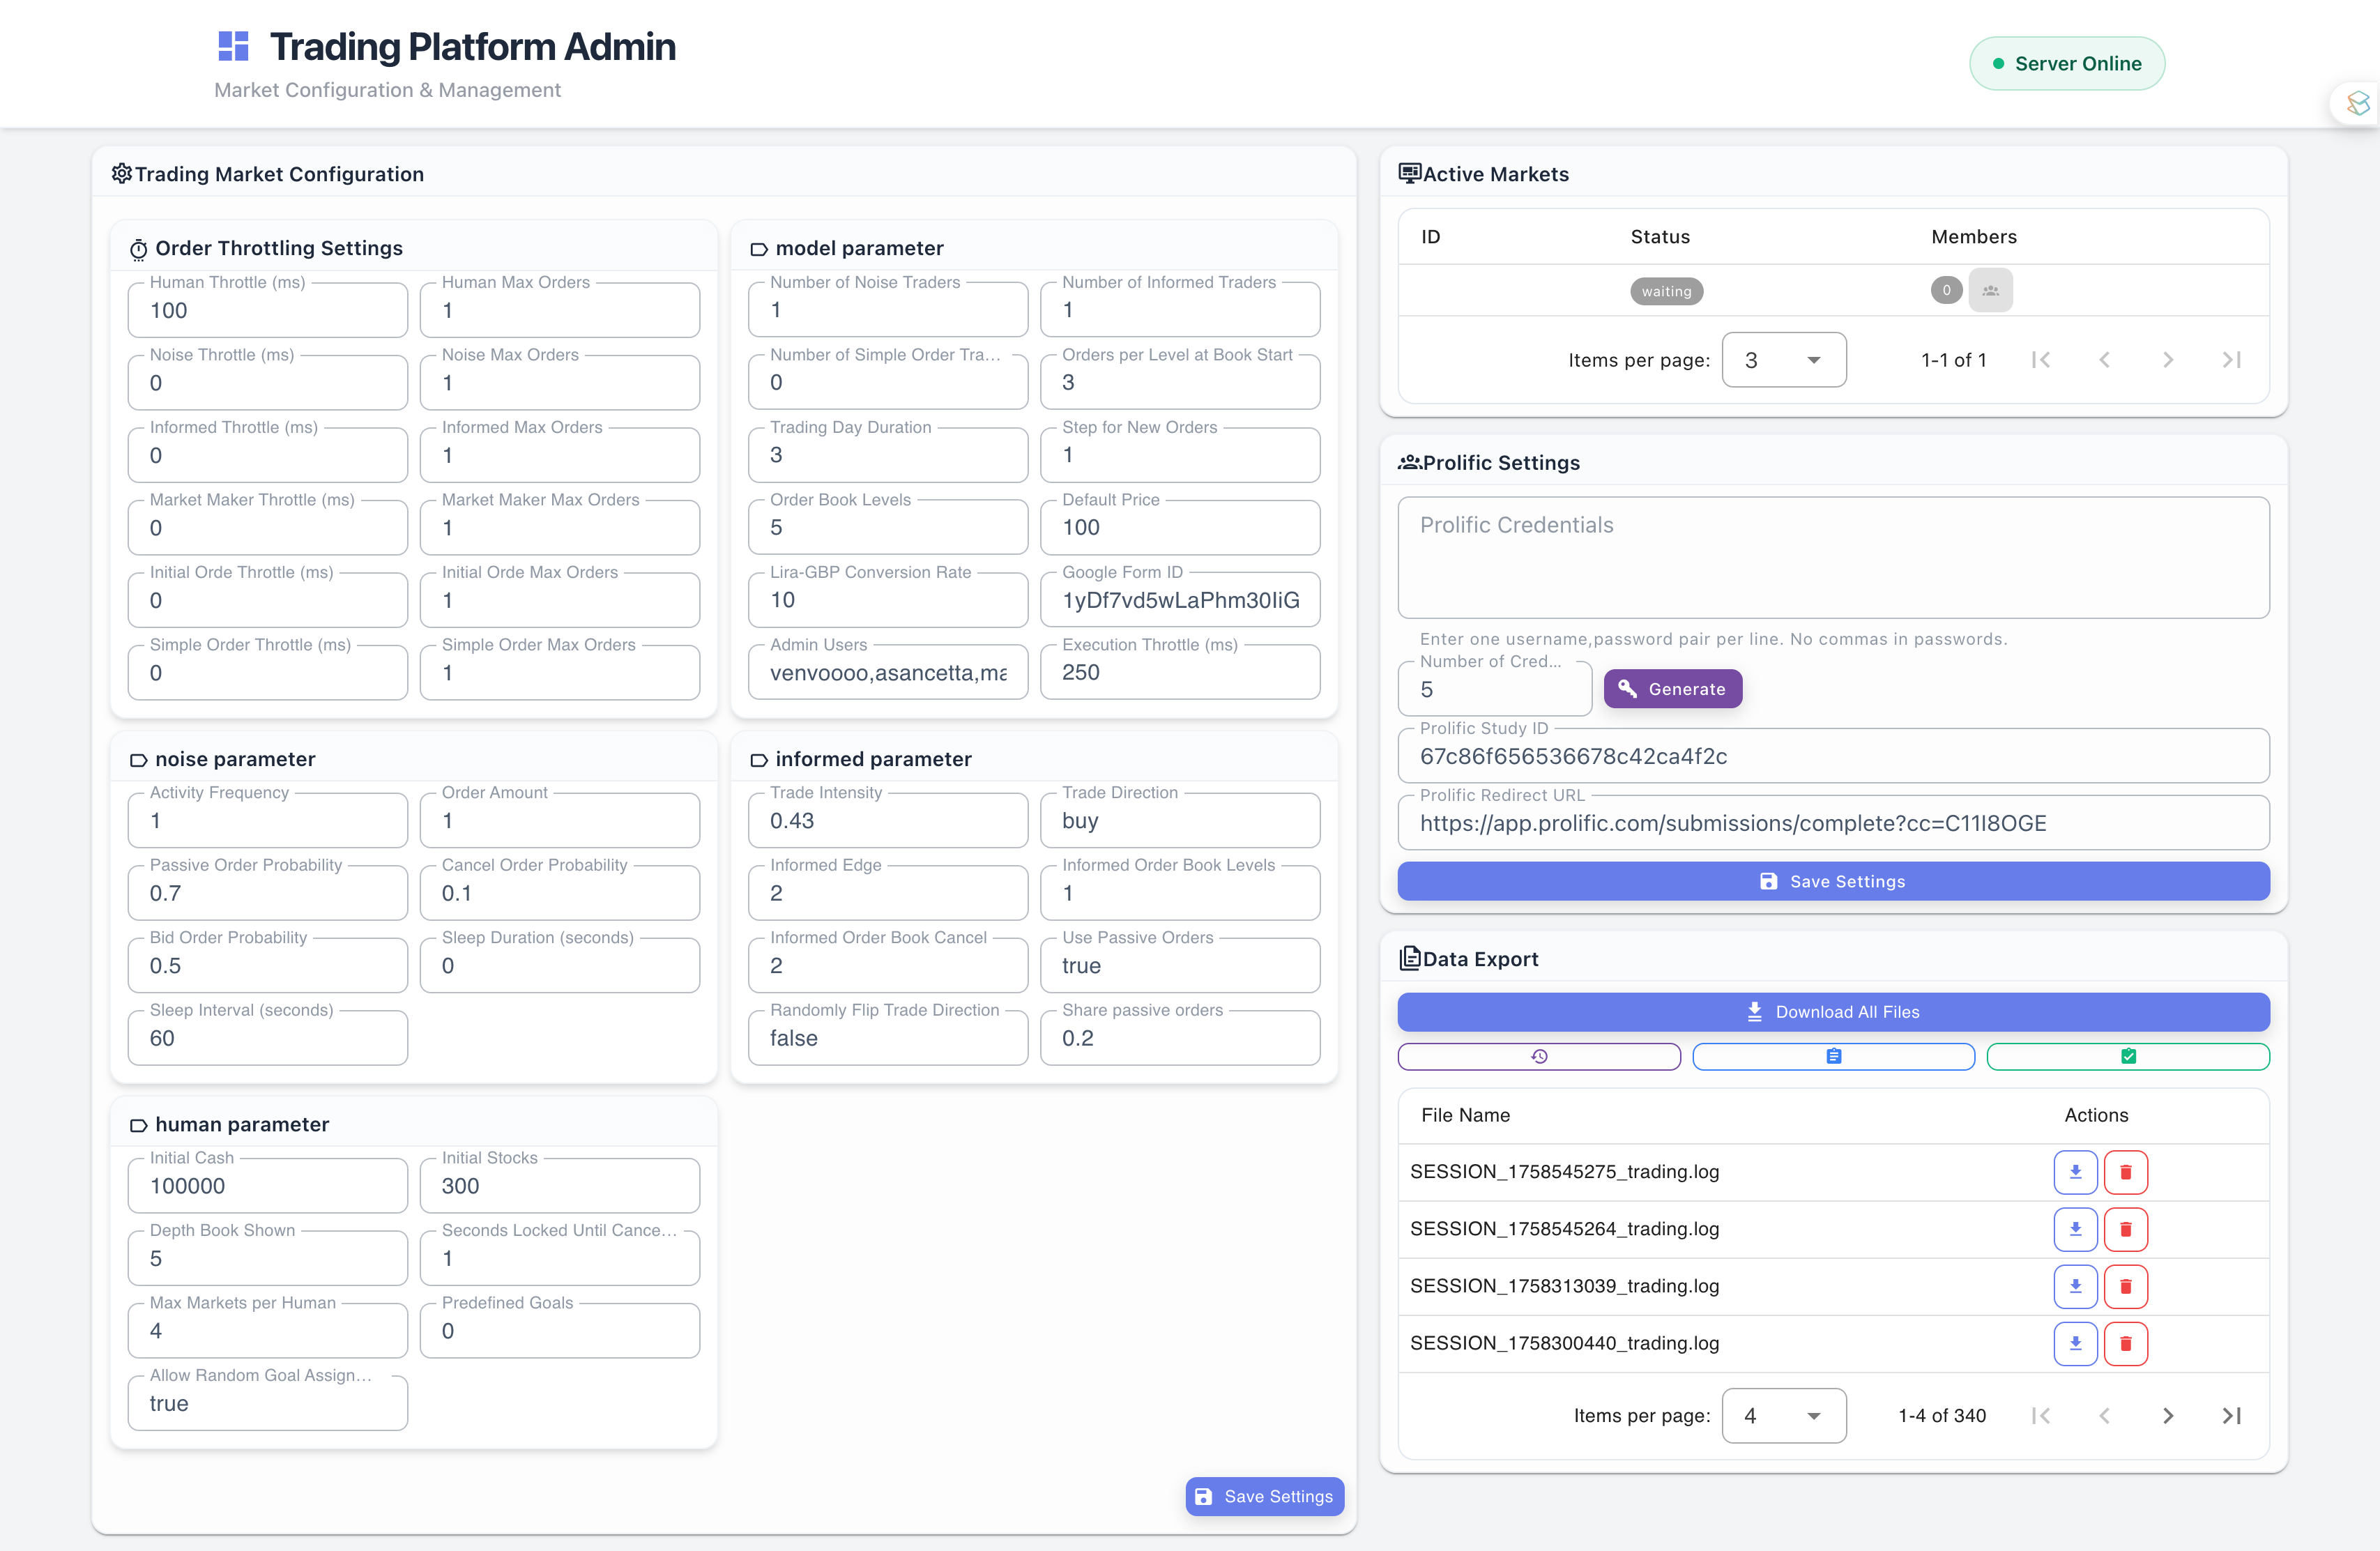
\includegraphics[width=0.95\textwidth]{figs/admin-page.png}
\caption{Administrative Interface Dashboard. Four main sections for market configuration with order throttling, active markets monitoring, Prolific integration, and data export.}
\label{fig:admin}
\end{figure}

The Trading Market Configuration panel organizes all the platform's settings into categories that match different trader types and market mechanisms. Parameters are grouped as model parameters (market structure), noise parameters (trader behavior), informed parameters (trader settings), and human parameters (participant endowments and interface settings). The interface highlights modified parameters $\theta_p \neq \theta_{p,default}$ to show which treatments differ from baseline conditions.

The Order Throttling section controls platform performance by limiting how fast different trader types can place orders. Each trader type gets throttling parameters $(\tau_{type}, \omega_{type})$ where $\tau_{type}$ is the milliseconds between orders and $\omega_{type}$ is the number of orders allowed per time window. This helps researchers balance realistic trading with computer system limitations.

The Active Markets Monitor shows the status of all parallel markets $\mathcal{M} = \{M_1, M_2, \ldots, M_j\}$ running at the same time. Each session entry shows how many participants have joined compared to how many are needed $|\mathcal{N}_j|/\nu_j$, the session status, and control buttons. The force-start feature lets researchers start markets even when they don't have enough participants, bypassing the normal wait-until-full rule when $|\mathcal{S}_s| < \nu_s$.

The Prolific Settings panel connects with research platforms by managing credentials and study settings. The platform creates and validates participant login information, manages study identifiers, and sets up redirect URLs for connecting with recruitment platforms like Prolific.

The Data Export section lets researchers download data for post-experiment analysis. The interface allows bulk data downloads, parameter history tracking, questionnaire response collection, and consent form management. File operations support data extraction while keeping data secure and protecting participant privacy.

\subsection{Trader Extensibility}
\label{sec:extensibility}

The platform lets researchers add new types of traders that work with all the market mechanisms we described above. This flexibility allows testing new behavioral models within controlled experimental environments.

\subsubsection{Basic Trader Setting}

All trader types are built on a common foundation that provides basic market interaction abilities. The platform automatically handles portfolio management $(C_{i,t}, S_{i,t})$, placing and canceling orders, communicating with the trading system, and tracking performance.

The platform uses standard communication methods. Each trader gets market updates including order book changes, trading session signals, market closure notifications, and transaction confirmations. The foundation provides standard behaviors that researchers can customize for specific trader types.

Order management follows the same procedures for all traders, including throttling limits, inventory updates, and platform communication. This makes sure all trader types operate under identical constraints and we collect consistent data.

The platform includes \texttt{SimpleOrderTrader} as an example that shows how to create custom trader types. This trader executes predetermined order sequences, giving researchers a concrete example of how to extend the basic trader framework.

\subsubsection{Shared Trading Environment}

All trader types have the same market access and face the same constraints. Each trader $i$ keeps track of their portfolio $(C_{i,t}, S_{i,t})$ and gets identical market information including the current order book state $(\mathbf{B}_t, \mathbf{A}_t)$, midpoint $p_{mid,t}$, and transaction history. The platform applies order throttling $\theta_{throttle}$ equally to all trader types to keep the experiment fair.

New trader types get the same information stream as existing traders: order executions, book updates, and timing signals. Custom trader types work with the parallel market creation and timing coordination systems, allowing studies where new behavioral models interact with human participants. Data collection works identically for custom traders, creating event logs that integrate with our reconstruction procedures to contribute to complete market state reconstruction $X_t = (\mathbf{B}_t, \mathbf{A}_t, p_{mid,t}, s_t, V_t)$.

\subsubsection{Behavioral Design Space}

Researchers can create traders with behaviors that cover the full range of existing trader types. Trading frequency can range from the continuous activity of noise traders to the discrete decisions of human traders. Order placement can follow fixed rules like informed traders or random patterns like noise traders.

Custom traders can be flexible with goal assignments - they can receive specific objectives $g_i$ from the session pool system or operate without goals like noise traders. Starting resources can follow any of the established patterns: uniform $(C_0, S_0)$, unlimited $(C = \infty, S = \infty)$, or goal-matched allocations.

\subsubsection{Example: Spread-Narrowing Market Maker}

Here's an example of a custom trader that provides liquidity by placing orders within the current bid-ask spread to make the market tighter. This trader watches the current best bid $p_{bid,t} = \max(\mathbf{B}_t)$ and best ask $p_{ask,t} = \min(\mathbf{A}_t)$, then places orders at better prices within the spread.

The trader's order placement strategy follows:
\begin{align}
p_{new\_bid} &= p_{mid,t} - \nu \cdot \frac{s_t}{2} \\
p_{new\_ask} &= p_{mid,t} + \nu \cdot \frac{s_t}{2}
\end{align}
where $\nu \in (0,1)$ is the spread improvement factor, $s_t = p_{ask,t} - p_{bid,t}$ is the current bid-ask spread, and $p_{mid,t}$ is the current midpoint.

This trader operates with unlimited money and shares $(C = \infty, S = \infty)$ to avoid budget constraints and continuously places limit orders at the improved prices with unit quantities. When orders execute, the trader immediately places new orders to maintain market presence. The trader cancels existing orders when market conditions change, keeping orders competitive.

Trader types like this enable studies of liquidity provision effects where researchers can examine how spread-narrowing behavior affects market quality measures including bid-ask spreads $s_t$, market depth, and price discovery efficiency.

\newpage
% Include results and discussion
\section{Empirical Illustration}
In this section, we illustrate the capabilities of the MINT platform using data from a real experimental study. The empirical illustration is based on \cite{feri2026}, where the authors investigate the interaction between human and machine traders. Specifically, the paper investigates how volume-based information is disseminated in the markets, and whether human participants are able to acquire this information and employ a profitable trading strategy. The authors investigate trading behaviour under different treatments, including treatments where the machine informed traders reach their goal by using only aggressive orders, or scenarios where the machine informed trader uses a mixture of passive and aggressive orders to try and conceal their private information.

The experiments were conducted in June and July 2025, and participants were recruited via the Prolific platform. Each participant, participated in one session, where each session consisted of 6 markets\footnote{The first market was considered as a practise market, and was not taken into account for calculating the final reward.}. For illustration, we present the results from a randomly selected market. In this market, the platform configuration parameters are set as:
\begin{equation*}
\left\{ \tau=3, p_{0} = 100, \sigma=1, \mathbf{g}=[0], |\mathcal{A}_{N}| = 1, \delta = 0.7, \zeta=0.5, |\mathcal{A}_{I}| =1, \beta=0.43, \psi_{I} = \text{False}\right\}
\end{equation*}
The rest follow their default values, as presented in Appendix A, Table \ref{tab:parameters}.

Thus, in this market, a machine informed trader buys 40 shares using only aggressive orders. The human participant acts as a Speculator, and is therefore allowed to post both bid and ask orders, as well as passive and aggressive orders. Their goal is to maximise their profits. In addition, the noise trader posts bid and ask orders with probability 0.5, and sends aggressive orders with probability 0.3. As a result, their impact on expected final price is zero. Instead, the noise trader generates a white-noise effect on the price and exists solely to maintain some level of trading activity, ensure sufficient liquidity in the market.

Thus, the only forces that can shift the price are the trades executed by the machine informed trader and the human participant.
\subsection{Trading behaviour}
Following the above, Figure \ref{fig:empirical_midprice} shows how the market price evolved over the three minute trading activity. Specifically, Panel (a) shows the midprice evolution and Panel (b) illustrates the best bid price $\max(\mathbf{B}_t)$, the best ask price $\min(\mathbf{A}_t)$, as well as the informed trades. 

It is clear that the presence of the informed trader had a profound effect on the market, shifting the midprice by approximately 10 $\sigma$. As shown in Panel (b) of Figure \ref{fig:empirical_midprice}, the informed trader relied exclusively on aggressive orders, crossing the spread. In doing so, the informed trader effectively moved the market, as their trades consumed depleted liquidity at the best available ask orders and pushed both the bid and the ask price to new higher values. 

Thus, it is evident that the informed trader creates opportunities for employing various profitable strategies, such as buying shares early on and selling them later when both the ask and bid prices have risen significantly.
\begin{figure}[!htbp]
    \centering
    \subfloat[\centering Midprice]{{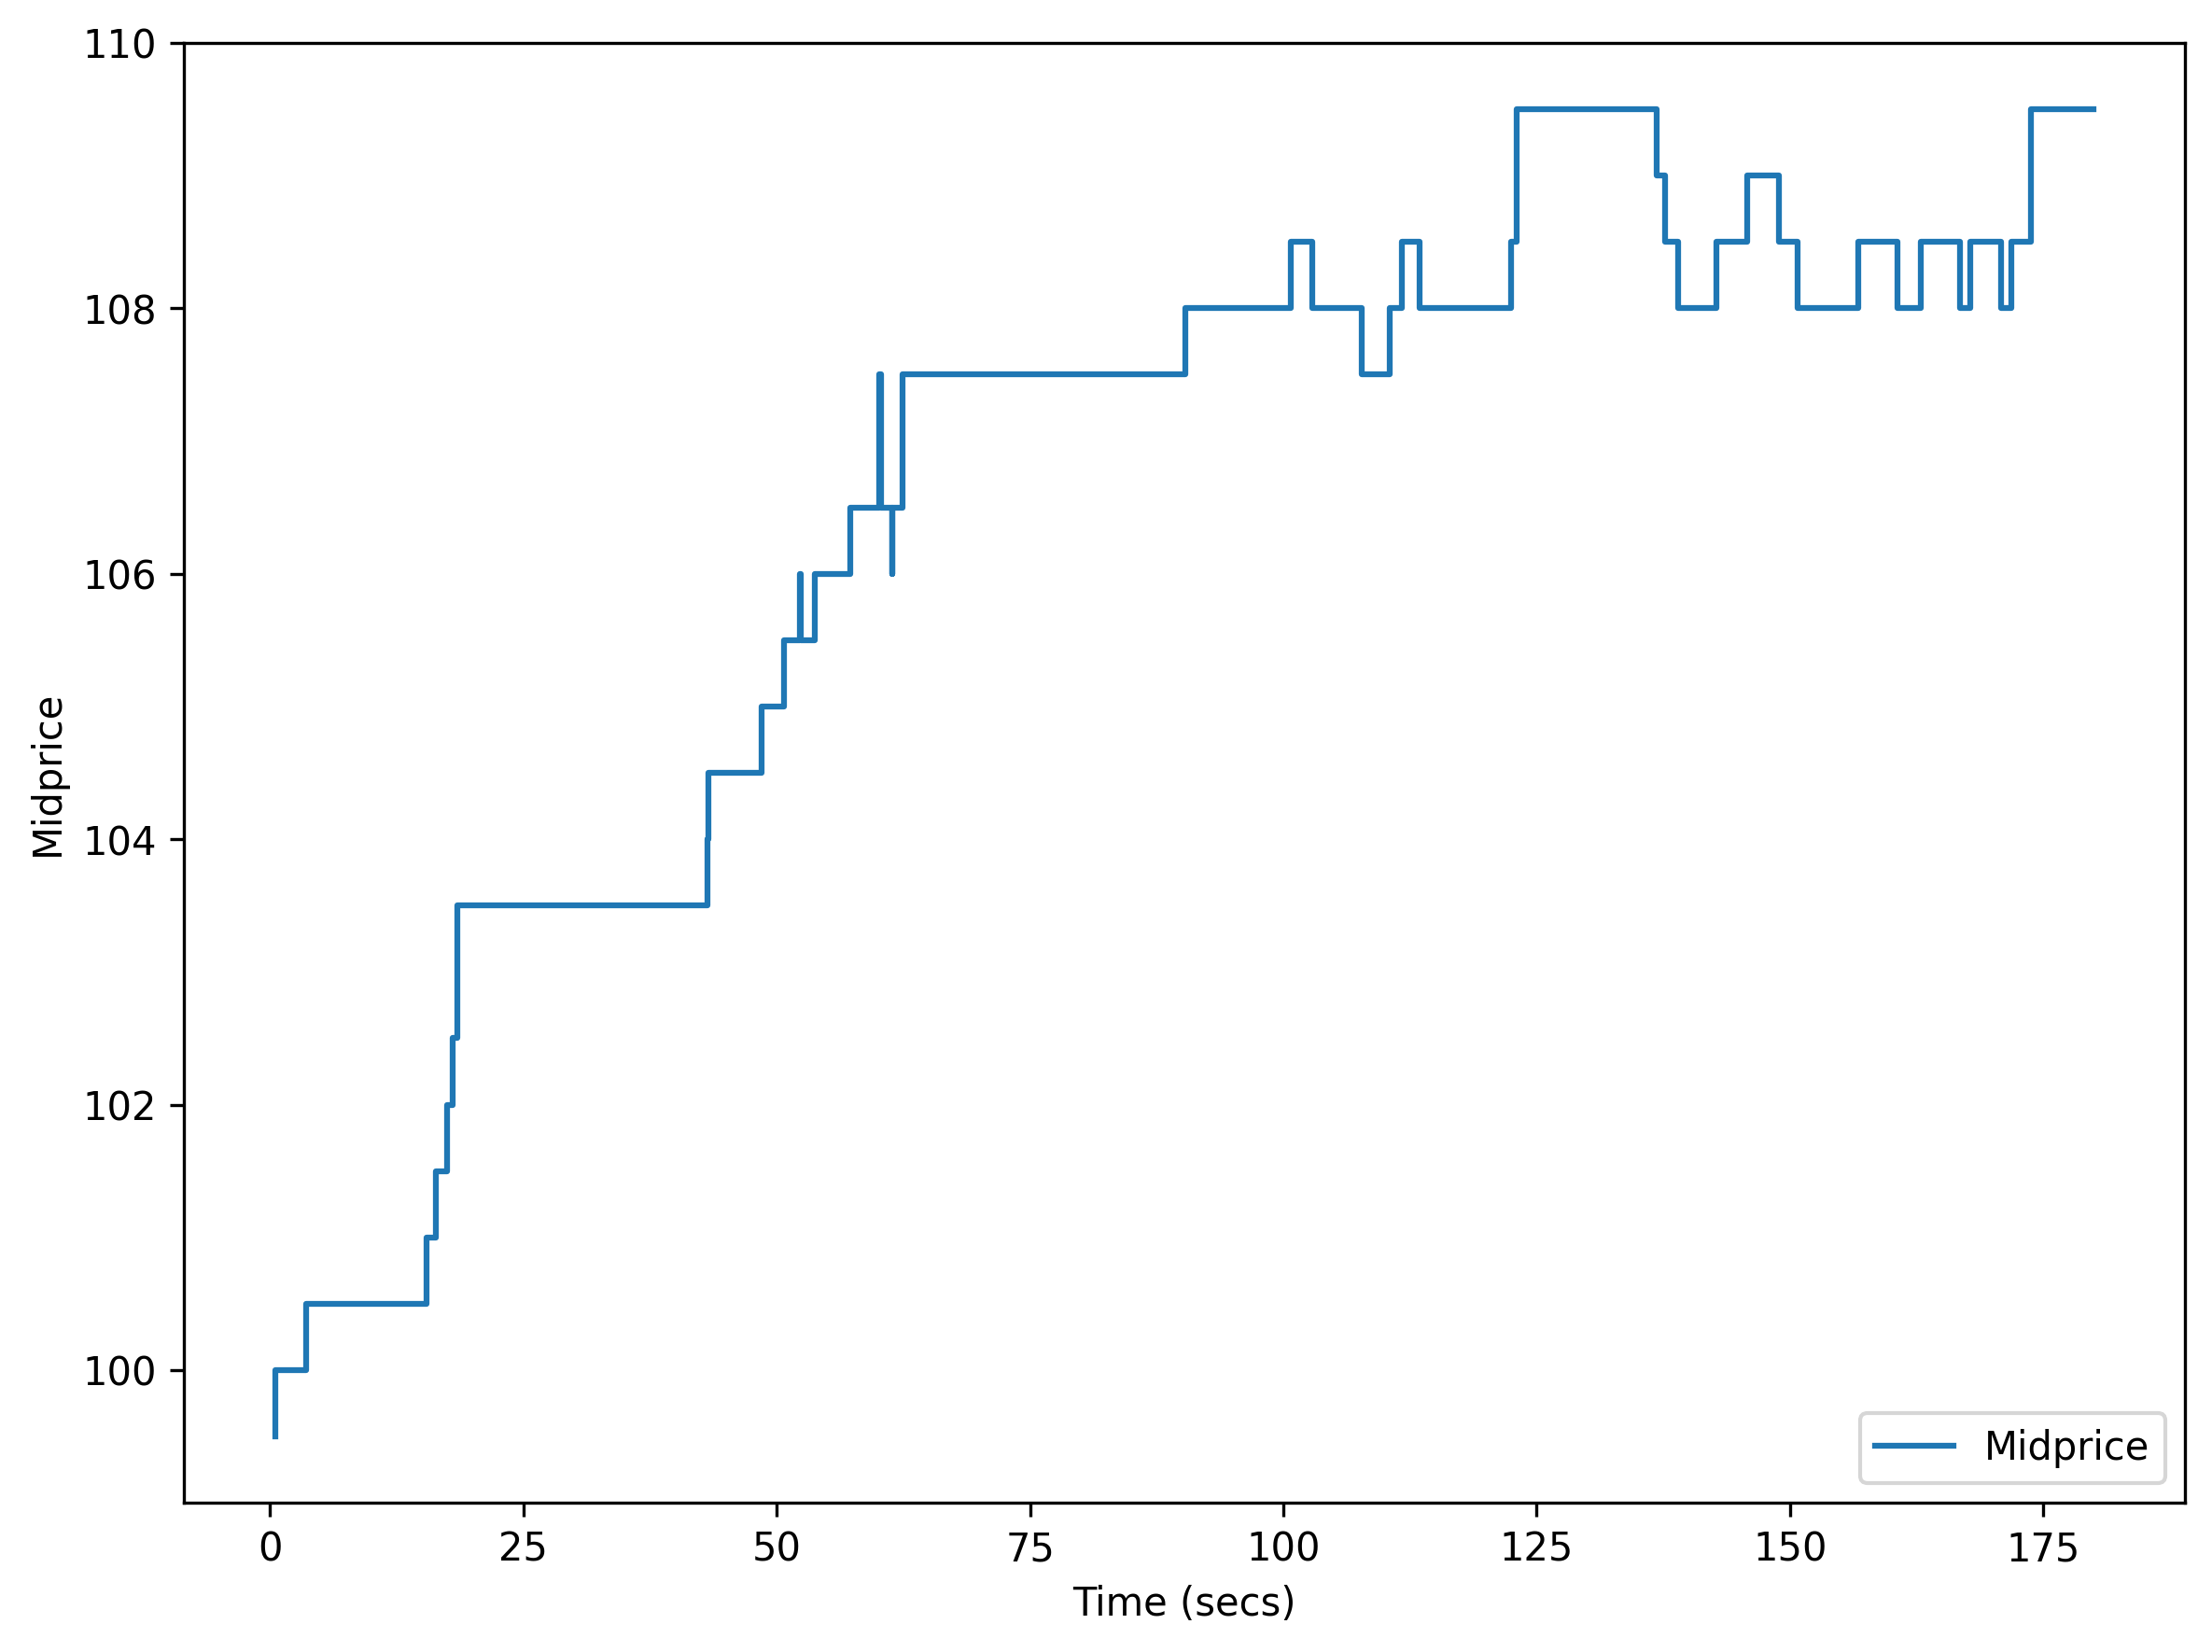
\includegraphics[scale=0.35]{figs/40_midprice.png} }}
    \qquad
    \subfloat[\centering Informed Trades]{{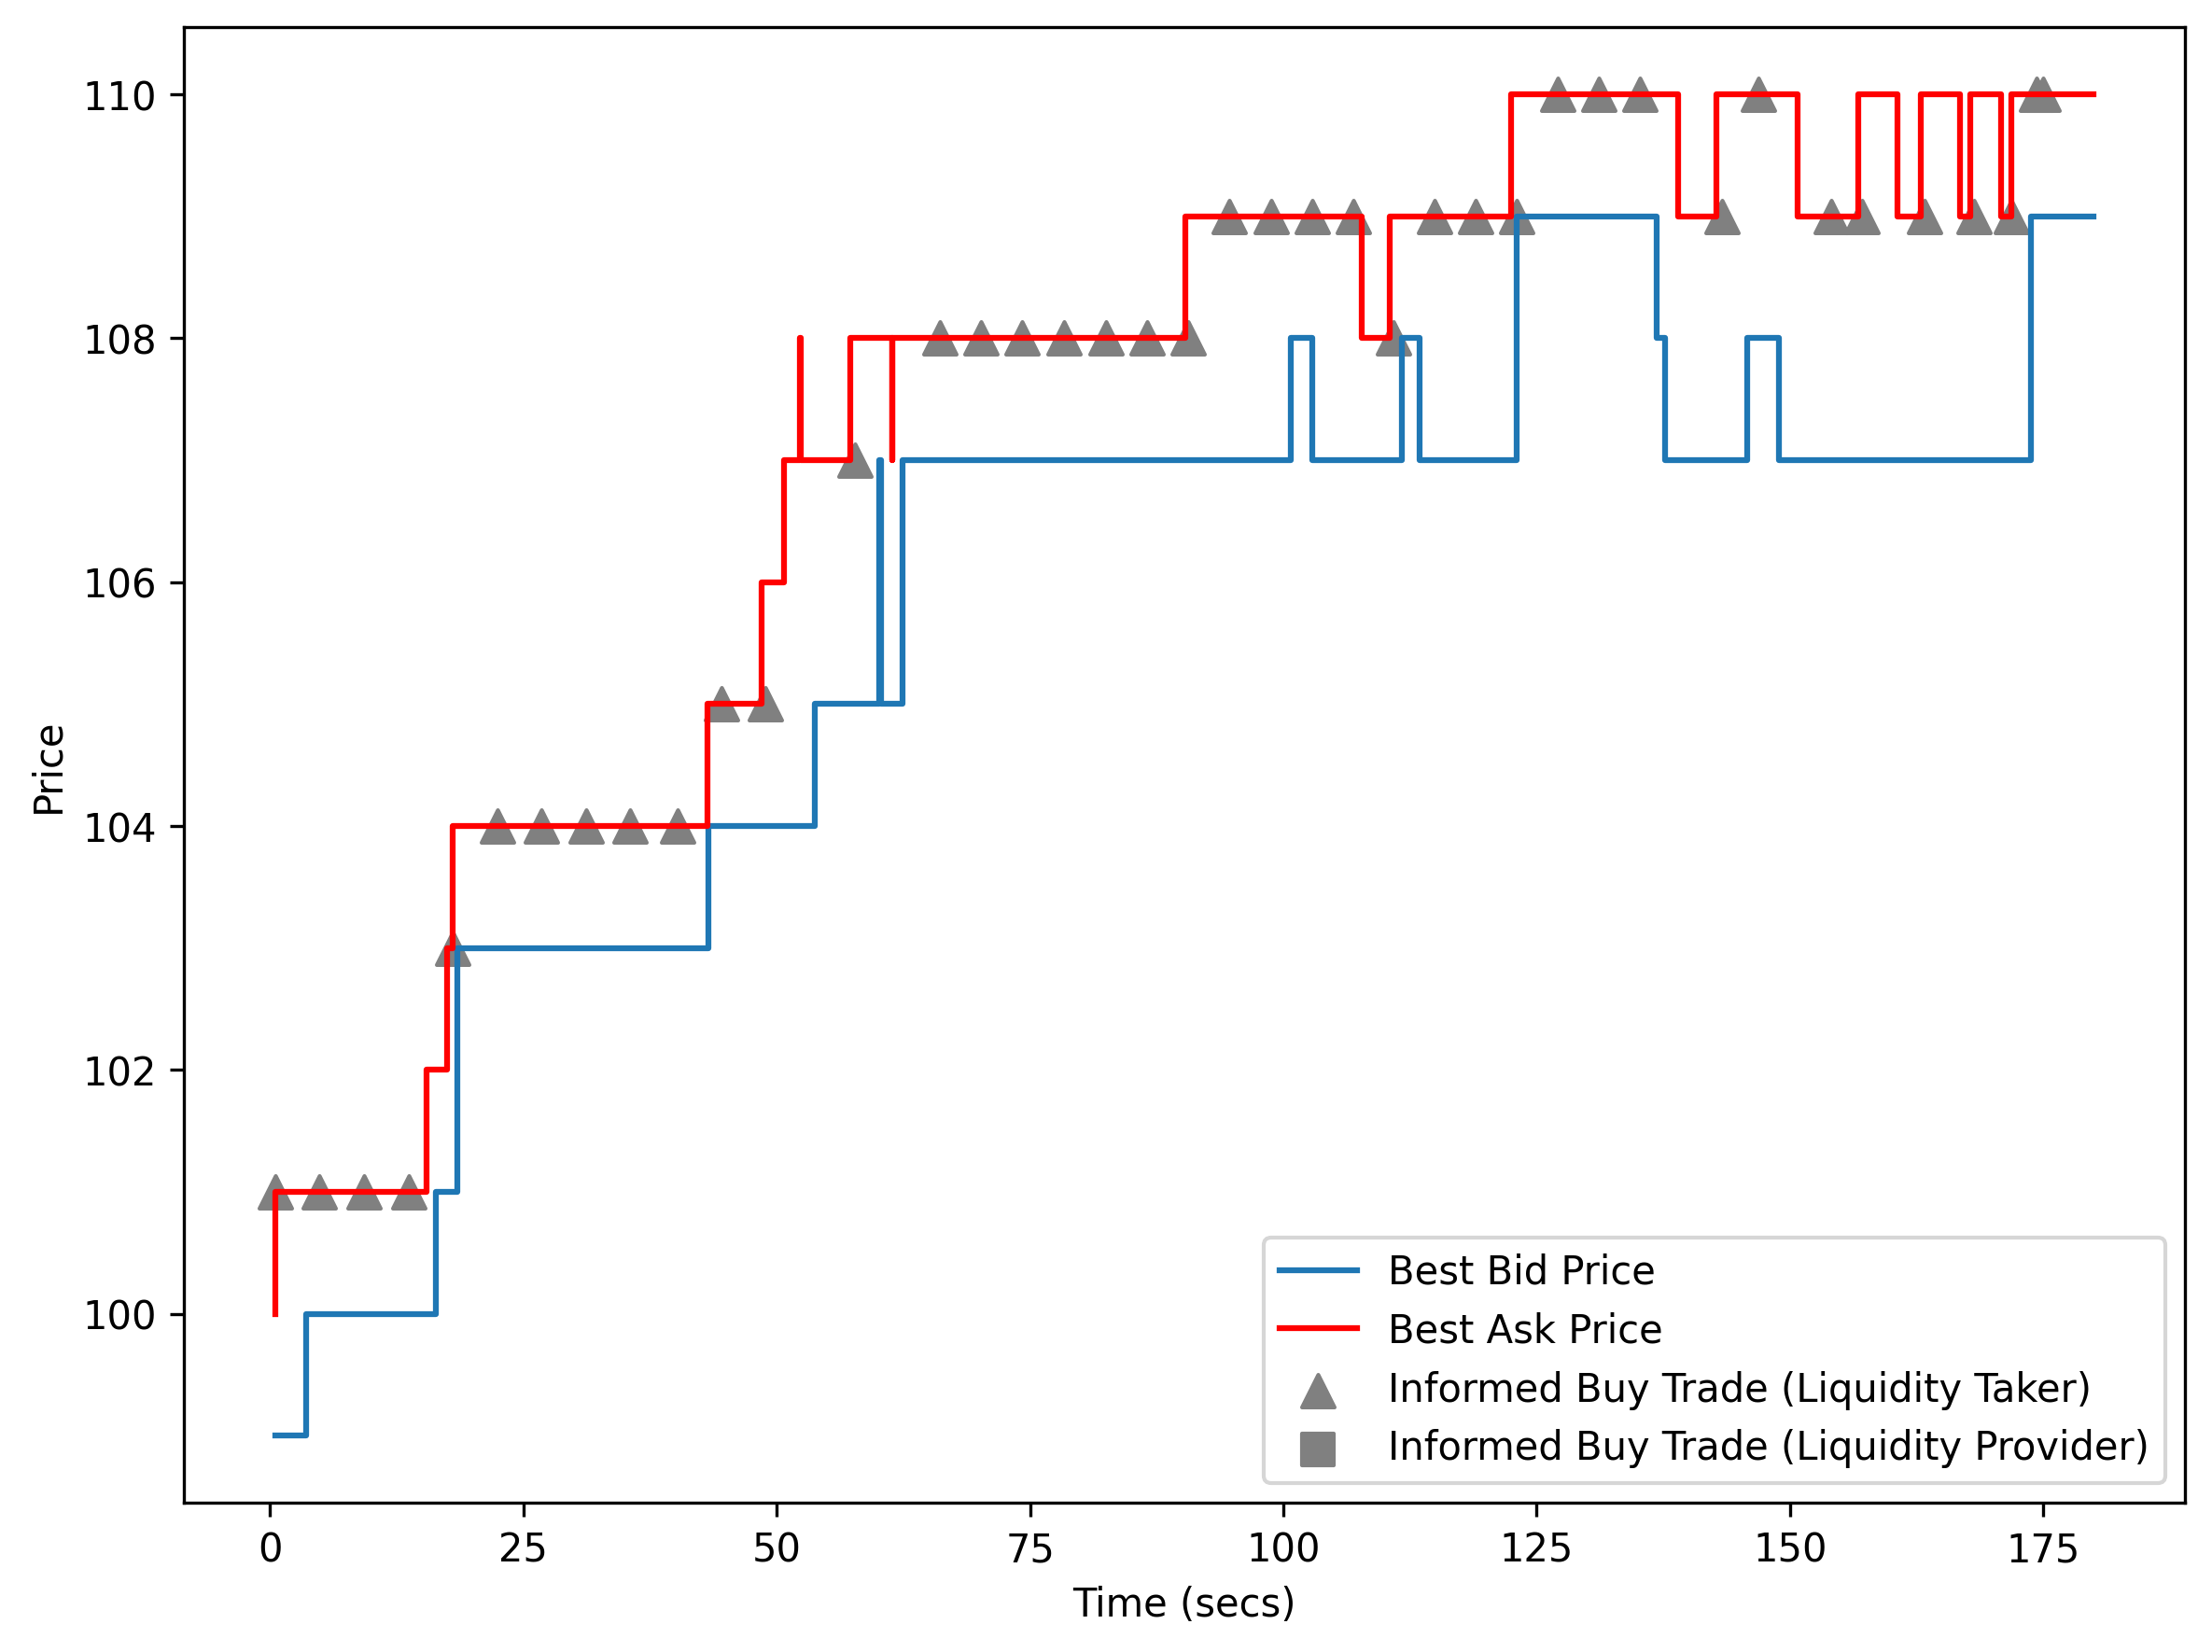
\includegraphics[scale=0.35]{figs/40_informed_trades.png} }}
    \caption{Midprice Evolution and Informed Trading}
    \label{fig:empirical_midprice}
\end{figure}

Next, we analyse the trading behaviour of the human participant. Figure \ref{fig:human_trading_activity} illustrates the trading activity of the participant, as well with their net inventory. Specifically, Panel (a) shows all the limit orders (bid and ask orders) sent by the participant. Panel (b) shows all the human trades classify them as Buy Trades and Sell Trades. Panel (c) depicts the net inventory over the three minutes period.
\begin{figure}[!htbp]
    \centering
    \subfloat[\centering Human Limit Orders]{{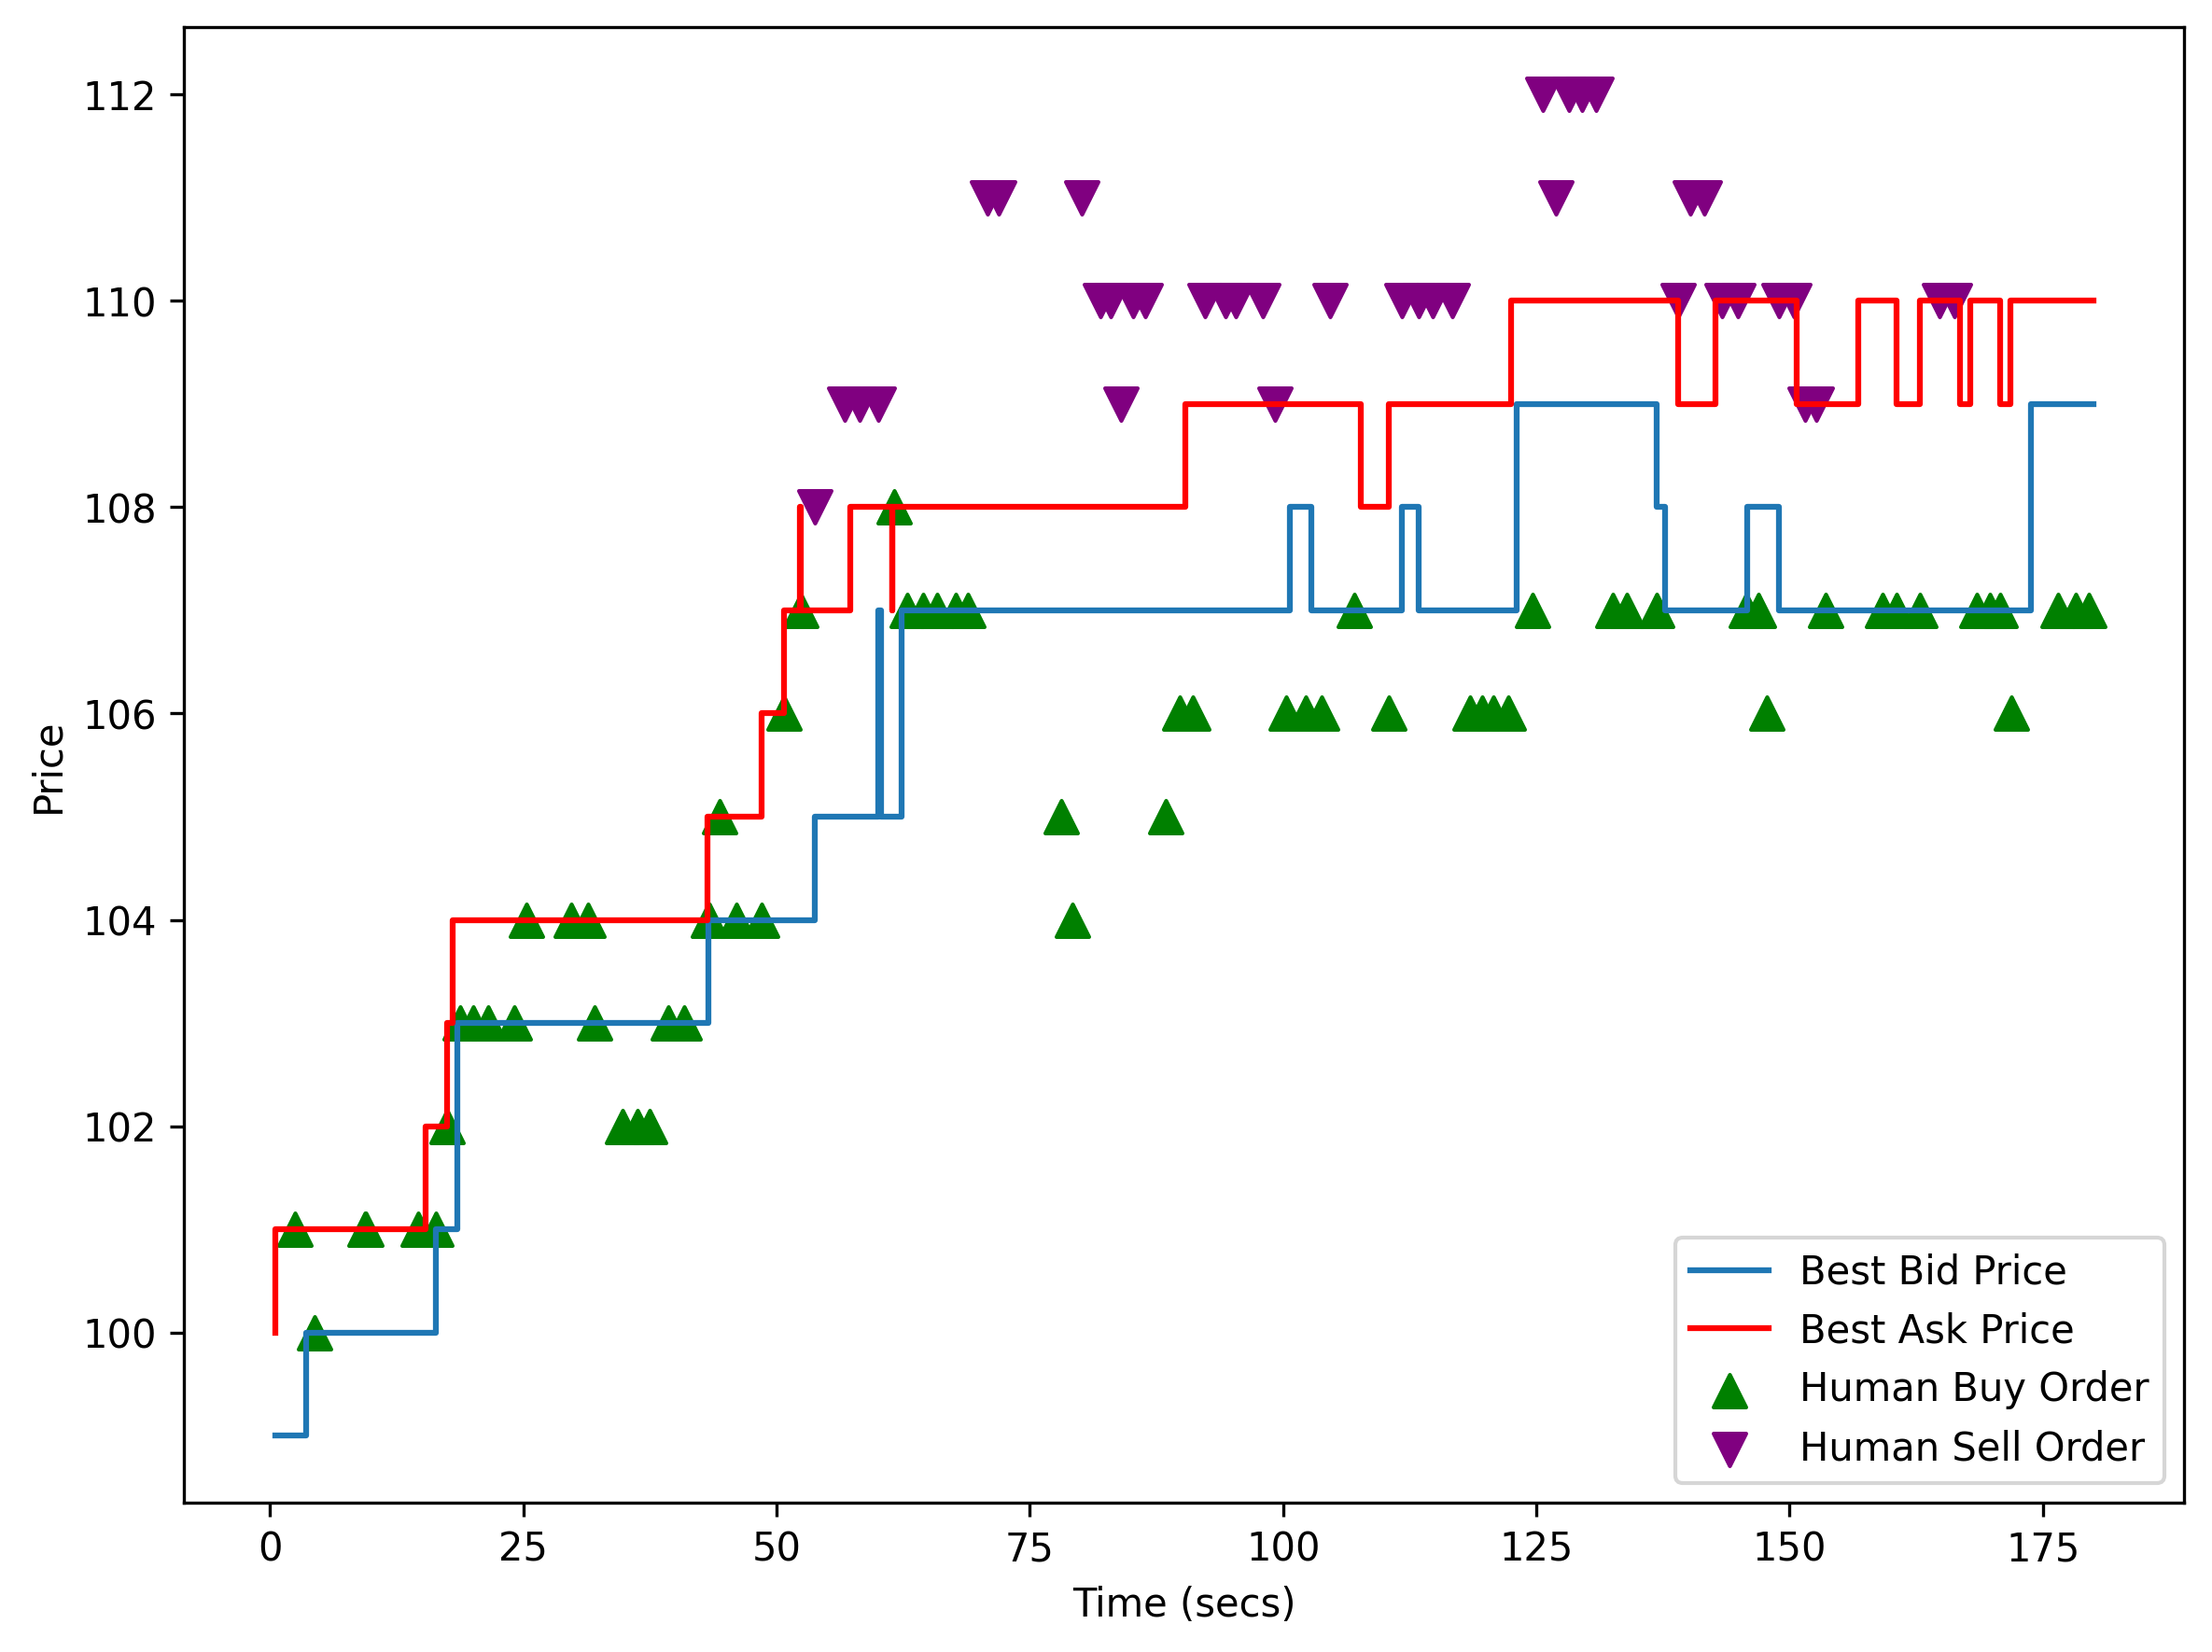
\includegraphics[scale=0.35]{figs/40_orders.png} }}
    \qquad
    \subfloat[\centering Human Trades]{{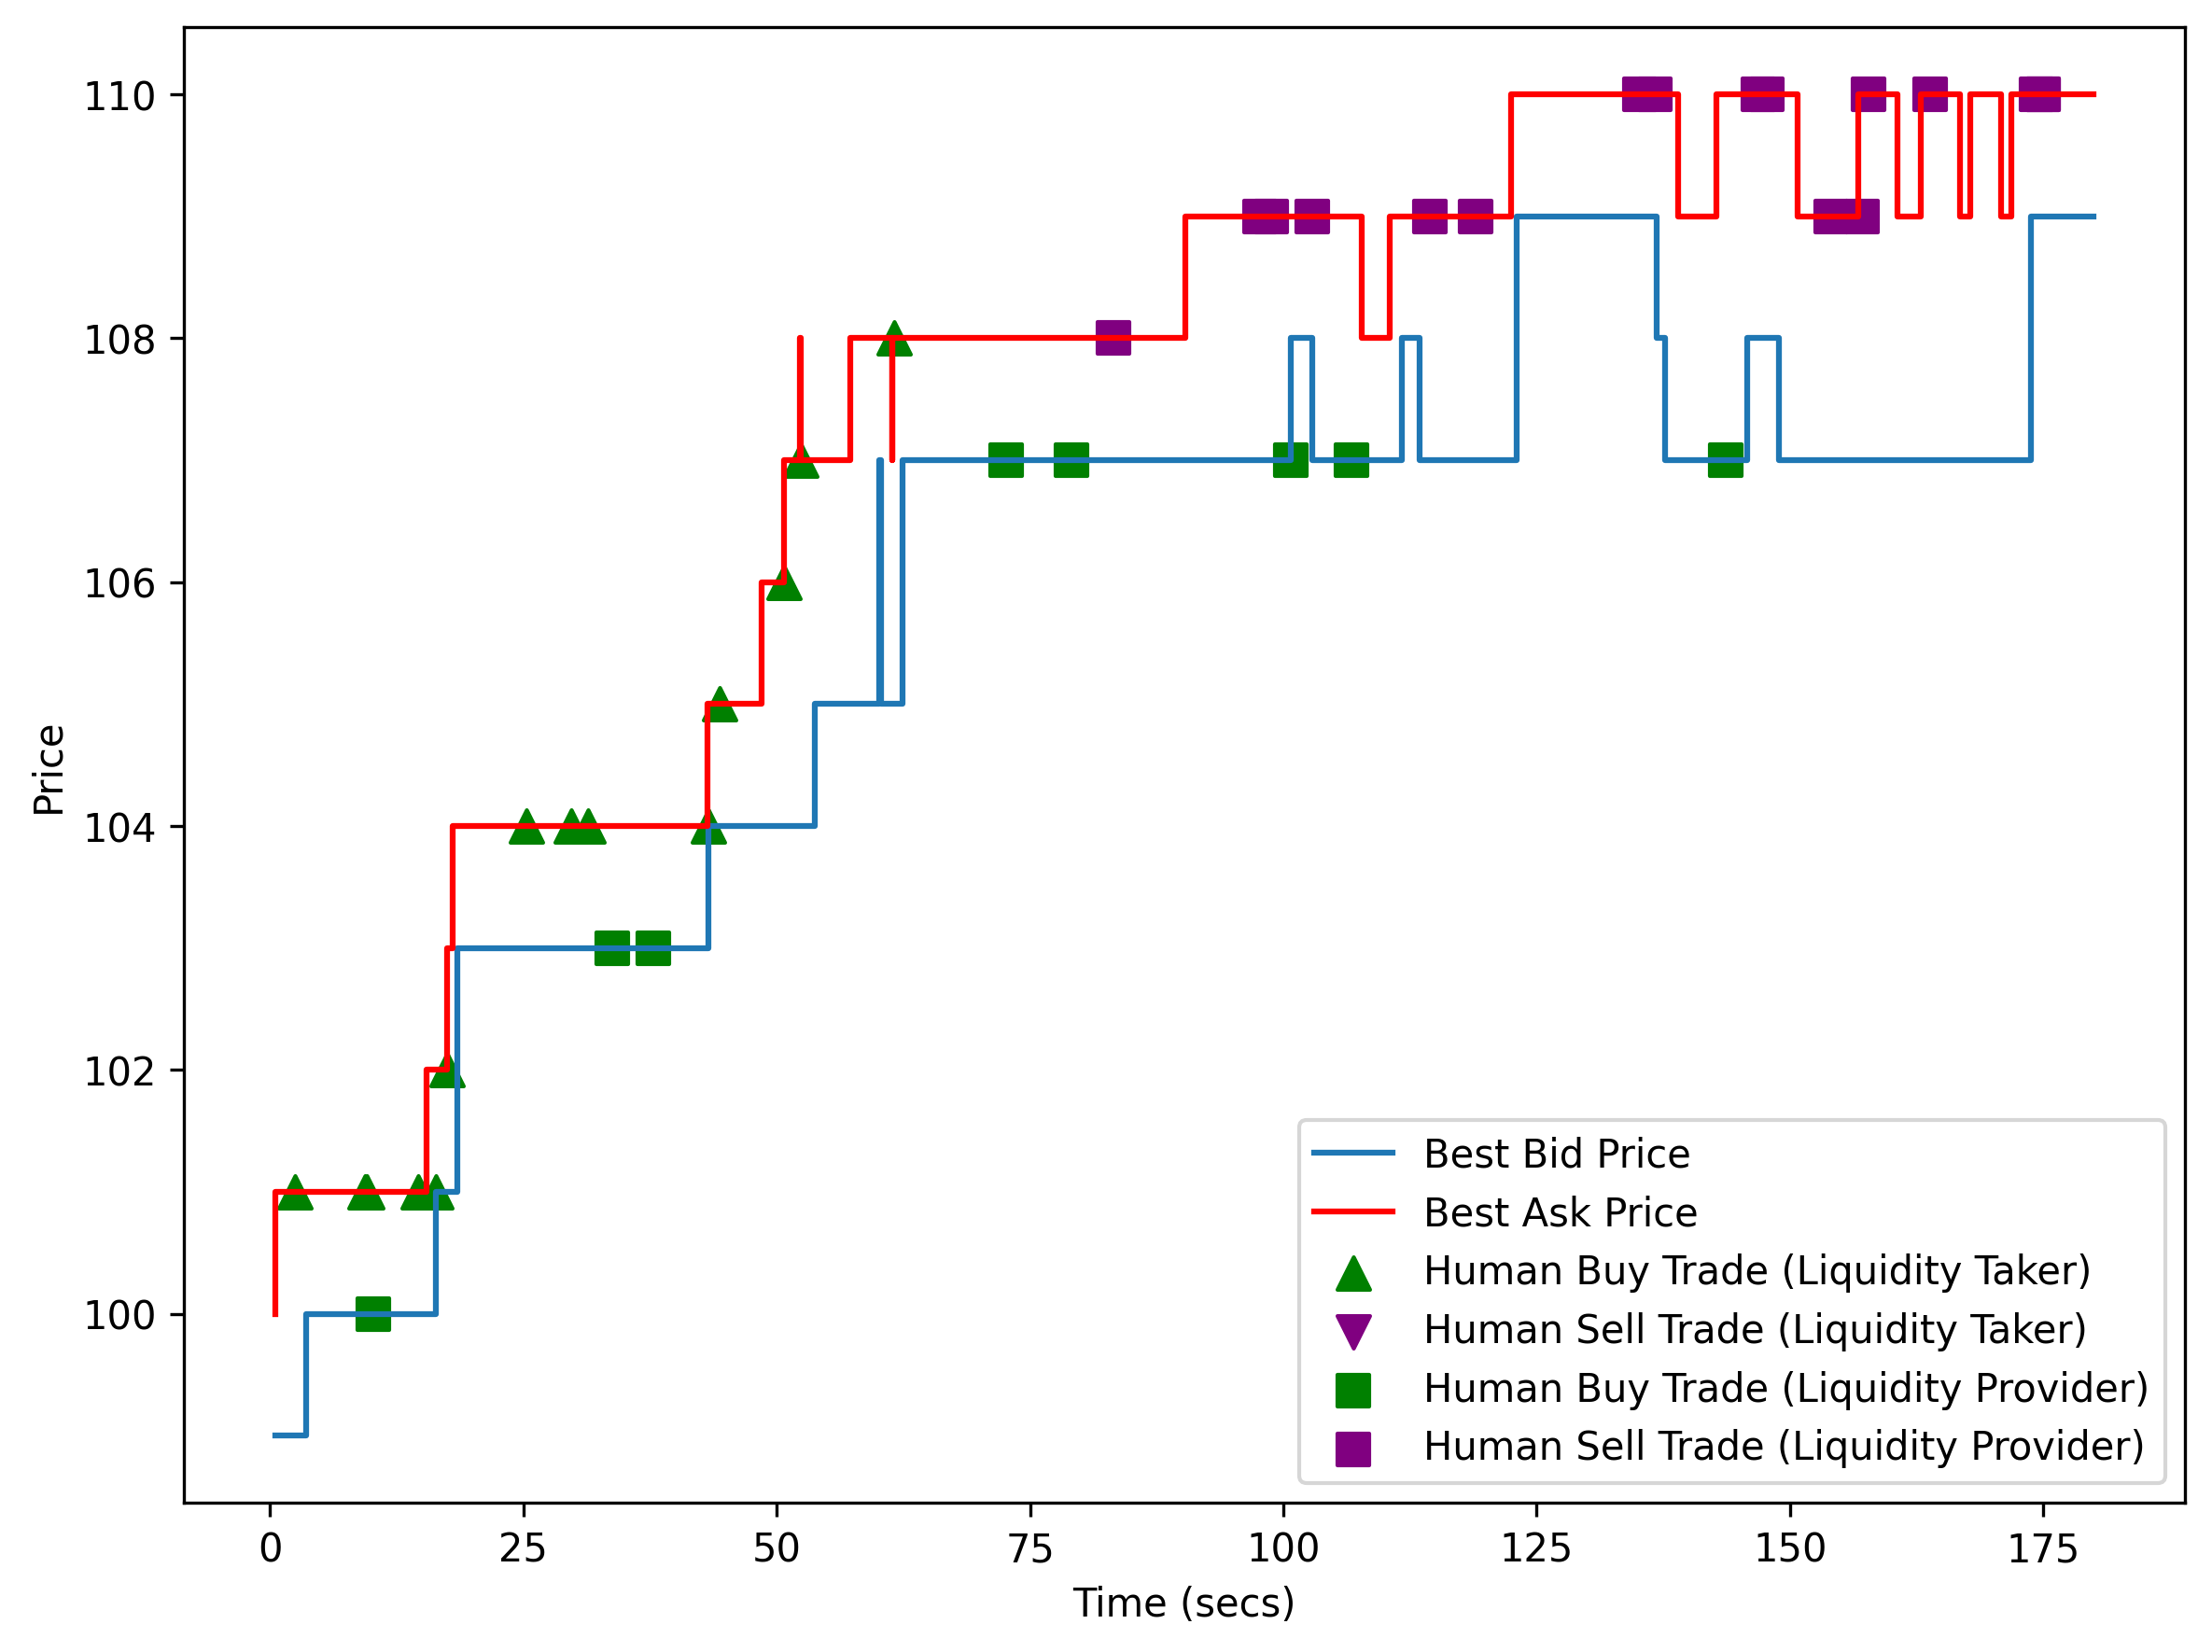
\includegraphics[scale=0.35]{figs/40_trades.png} }}
    \qquad
    \subfloat[\centering Human Net Inventory]{{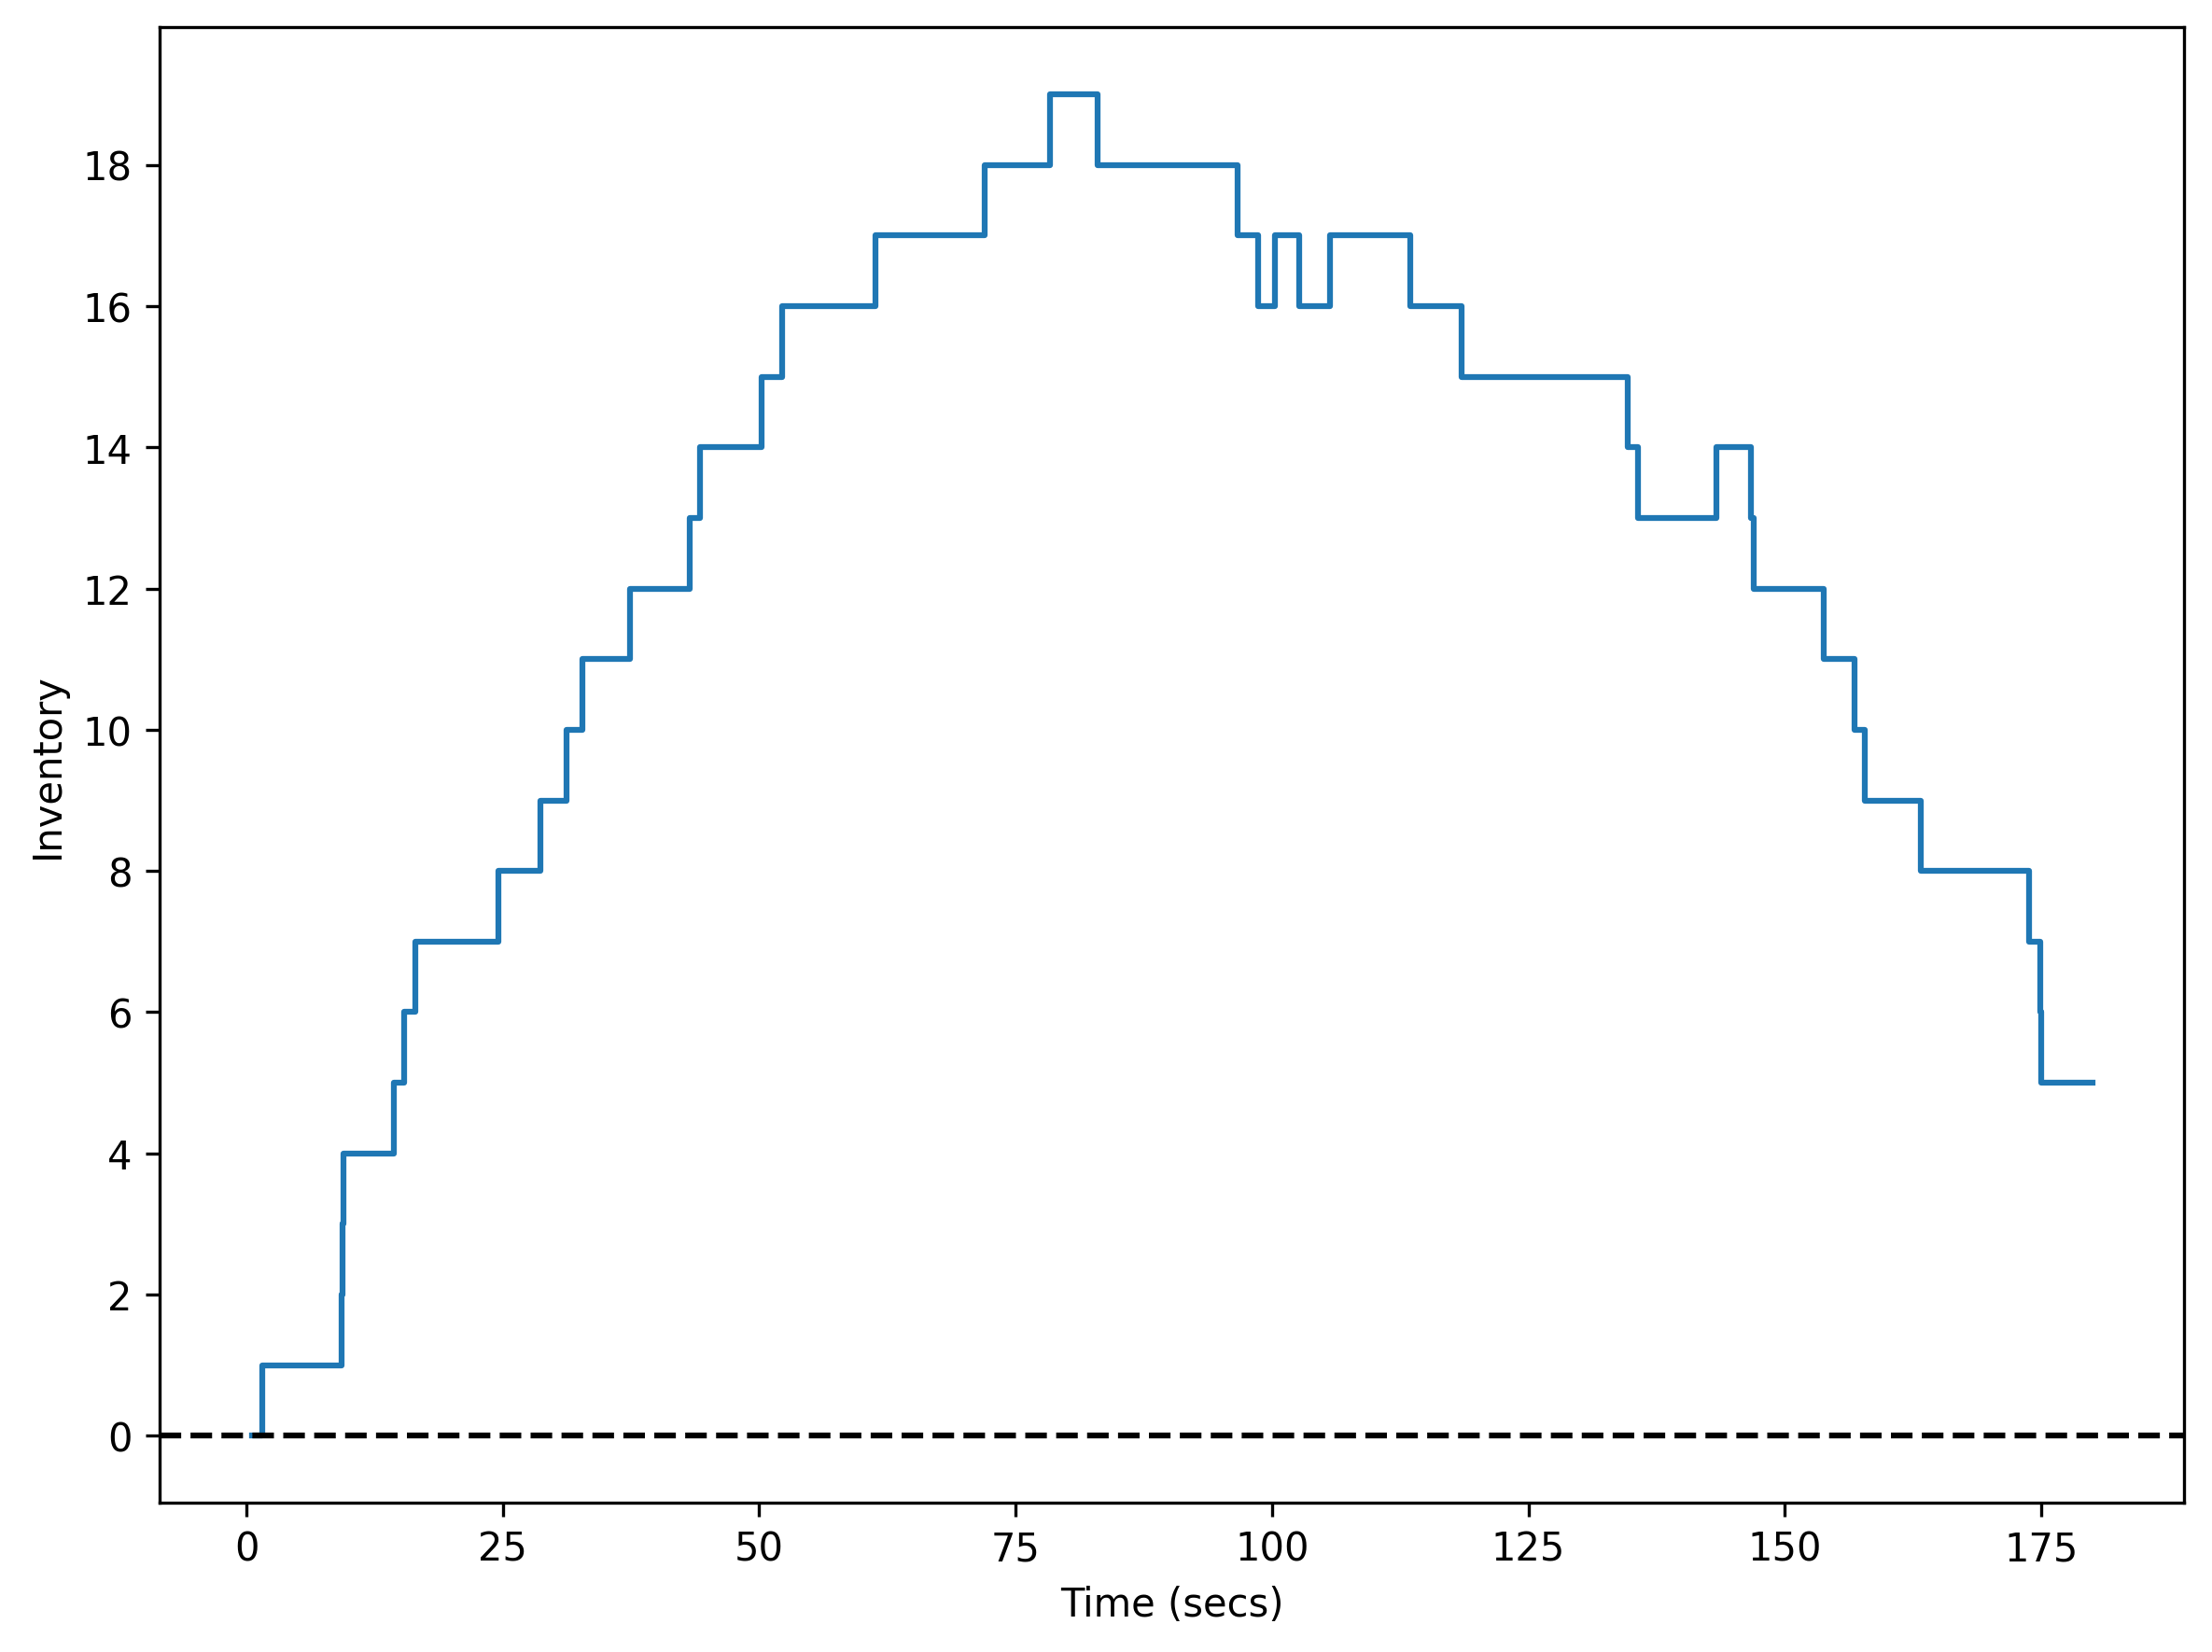
\includegraphics[scale=0.35]{figs/40_inv.png} }}
    \caption{Human Trading Activity}
    \label{fig:human_trading_activity}
\end{figure}

In addition, Table \ref{tab:empirical_human_trades} summarises the human's trades. Last we can see that the $VWAP_{buy} = 104.09$ and the $VWAP_{buy} = 107.32$ , indicating that the participant managed to deploy a profitable strategy. Here, we want to highlight that the last 5 orders at the Sell Trades column, consist of the automated platform orders which balanced the net inventory. 

It is interesting that even thought the participant din't manage to exit the market with a balanced net inventory, in this specific market, the penalisation of the platform, didn't affect much their profitability, and such, the participant managed to make a $PnL = 71$.
\begin{table}[h]
\centering
\caption{Summary of Human Buy and Sell Trades}
\label{tab:empirical_human_trades}
\begin{tabular}{cc|cc}
\toprule
\multicolumn{2}{c|}{Buy Trades} & \multicolumn{2}{c}{Sell Trades}\\
Quantity & Price  & Quantity & Price  \\
\hline
1 & 100 & 1 & 108\\
5 & 101 & 7 & 109\\
1 & 102  & 9 & 110\\
2 & 103  & 5 & 100\\
4 & 104 \\
1 & 105 \\
1 & 106 \\
6 & 107 \\
1 & 108 \\
\hline
Num. Trades & 22 & Num. Trades & 22  \\
Total Spent & 2290 & Total Received & 2361\\
VWAP & 104.09 & VWAP & 107.32  \\
\bottomrule
\end{tabular}
\end{table}

\subsection{Additional Order Book Metrics}


\section{Discussion and Future Directions}


\subsection{Backend-End}

\subsection{Front-End}


% Include conclusion
\section{Concluding Remarks}


\newpage
% Acknowledgements and Disclosure of Funding
\acks{
We thank the participants of the 3rd London Behavioural and Experimental Workshop for their valuable feedback on platform design and implementation. We acknowledge the contributions of the open-source community and the developers of the underlying technologies that made this platform possible. The authors acknowledge financial support from the Leverhulme Trust Grant Award PRG-2021-359.}

% Include appendix
\appendix

\section{Default Parameter Values}
\label{app:parameters}

Table \ref{tab:parameters} presents the complete set of configurable parameters with their example values, organized by functional category.

\begin{table}[h]
\centering
\caption{Platform Configuration Parameters}
\label{tab:parameters}
\begin{tabular}{p{0.15\textwidth}p{0.65\textwidth}r}
\toprule
Symbol & Description & Example \\
\midrule
\multicolumn{3}{l}{\textbf{Market Structure}} \\
$\tau$ & Market duration (minutes) & 3.0 \\
$p_0$ & Default starting price & 100 \\
$\ell$ & Order book depth levels & 5 \\
$\sigma$ & Price tick size & 1 \\
$\omega$ & Orders per level at initialization & 3 \\
\midrule
\multicolumn{3}{l}{\textbf{Human Trader Settings}} \\
$C_0$ & Starting cash endowment & 100,000 \\
$S_0$ & Starting share holdings & 300 \\
$\ell_{display}$ & Order book depth displayed & 5 \\
$\mu_{max}$ & Participation limit & 4 \\
$\mathbf{g}$ & Predefined goals vector & [0] \\
$\chi_{random}$ & Allow random goal assignment & True \\
\midrule
\multicolumn{3}{l}{\textbf{Noise Trader Settings}} \\
$|\mathcal{A}_N|$ & Number of noise traders & 1 \\
$\alpha$ & Actions per minute & 1.0 \\
$q_{max}$ & Maximum order size & 1 \\
$\delta$ & Passive order probability & 0.7 \\
$\epsilon$ & Order cancellation rate & 0.1 \\
$\zeta$ & Bid order probability & 0.5 \\
$\rho_{sleep}$ & Sleep duration (seconds) & 0 \\
$\phi_{sleep}$ & Sleep interval (seconds) & 60 \\
\midrule
\multicolumn{3}{l}{\textbf{Informed Trader Settings}} \\
$|\mathcal{A}_I|$ & Number of informed traders & 1 \\
$\beta$ & Trade intensity parameter & 0.43 \\
$\gamma$ & Pricing edge advantage & 2 \\
$\ell_I$ & Order book levels used & 1 \\
$\eta_I$ & Cancellation parameter & 2 \\
$\psi_I$ & Use passive order strategy & True \\
$\chi_I$ & Random direction assignment & False \\
$\xi_I$ & Share of passive orders & 0.2 \\
\midrule
\multicolumn{3}{l}{\textbf{System Settings}} \\
$\theta_{throttle}$ & Order processing throttle (ms) & 250 \\
$\lambda_{convert}$ & Currency conversion rate & 10 \\
$\Delta$ & Default spread width & 10 \\
$\kappa$ & Punishing constant & 1 \\
$\phi_{cancel}$ & Order lock duration (seconds) & 1 \\
$\Theta_{throttle}$ & Throttle settings per trader type & Complex \\
\bottomrule
\end{tabular}
\end{table}

These parameters enable researchers to customize market structure, trader behavior, and experimental conditions while maintaining system stability and realistic market dynamics.


\vskip 0.2in
\bibliography{references}

\end{document}
